%%%%%%%% ICML 2026 EXAMPLE LATEX SUBMISSION FILE %%%%%%%%%%%%%%%%%

\documentclass{article}

% Recommended, but optional, packages for figures and better typesetting:
\usepackage{microtype}
\usepackage{graphicx}
\usepackage{subcaption}
\usepackage{booktabs} % for professional tables
\usepackage{xspace}
\usepackage{svg}

% Algorithms (ICML recommends algorithm + algorithmic).
\usepackage{algorithm}
\usepackage{algorithmic}

% Citations (ICML uses natbib; icml2026 may load it, but include explicitly for consistency).
\usepackage{natbib}

% Small helpers used in the ICML example for table spacing.
\newcommand{\abovespace}{\vskip 0.10in}
\newcommand{\belowspace}{\vskip -0.10in}

% hyperref makes hyperlinks in the resulting PDF.
% If your build breaks (sometimes temporarily if a hyperlink spans a page)
% please comment out the following usepackage line and replace
% \usepackage{icml2026} with \usepackage[nohyperref]{icml2026} above.
\usepackage{hyperref}


% Attempt to make hyperref and algorithmic work together better:
\providecommand{\theHalgorithm}{\arabic{algorithm}}

% Use the following line for the initial blind version submitted for review:
\usepackage{icml2026}

% For preprint, use
% \usepackage[preprint]{icml2026}

% If accepted, instead use the following line for the camera-ready submission:
% \usepackage[accepted]{icml2026}

\usepackage{amsmath}
\usepackage{amssymb}
\usepackage{mathtools}
\usepackage{amsthm}


% if you use cleveref..
\usepackage[capitalize,noabbrev]{cleveref}

%%%%%%%%%%%%%%%%%%%%%%%%%%%%%%%%
% THEOREMS
%%%%%%%%%%%%%%%%%%%%%%%%%%%%%%%%
\theoremstyle{plain}
\newtheorem{theorem}{Theorem}[section]
\newtheorem{proposition}[theorem]{Proposition}
\newtheorem{lemma}[theorem]{Lemma}
\newtheorem{corollary}[theorem]{Corollary}
\theoremstyle{definition}
\newtheorem{definition}[theorem]{Definition}
\newtheorem{assumption}[theorem]{Assumption}
\theoremstyle{remark}
\newtheorem{remark}[theorem]{Remark}

% Todonotes is useful during development; simply uncomment the next line
%    and comment out the line below the next line to turn off comments
%\usepackage[disable,textsize=tiny]{todonotes}
\usepackage[textsize=tiny]{todonotes}
% The \icmltitle you define below is probably too long as a header.
% Therefore, a short form for the running title is supplied here:
\icmltitlerunning{POLAR-SGD: Efficient Cross-Datacenter Training via Prefix-based Communication Overlap and Error Correction}


\newcommand{\sysname}{POLAR-SGD\xspace}
\newcommand{\wang}{\textcolor{blue}}
\newcommand{\liao}{\textcolor{blue}}
\newcommand{\marked}{\textcolor{red}}

\begin{document}

\twocolumn[
  \icmltitle{POLAR-SGD: Efficient Cross-Datacenter Training via Prefix-based Communication Overlap and Error Correction}

  % It is OKAY to include author information, even for blind submissions: the
  % style file will automatically remove it for you unless you've provided
  % the [accepted] option to the icml2026 package.

  % List of affiliations: The first argument should be a (short) identifier you
  % will use later to specify author affiliations Academic affiliations
  % should list Department, University, City, Region, Country Industry
  % affiliations should list Company, City, Region, Country

  % You can specify symbols, otherwise they are numbered in order. Ideally, you
  % should not use this facility. Affiliations will be numbered in order of
  % appearance and this is the preferred way.
  \icmlsetsymbol{equal}{*}

  \begin{icmlauthorlist}
    \icmlauthor{Yuntong Li}{equal,bhu}
    \icmlauthor{Xiaojian Liao}{equal,bhu}
    \icmlauthor{Jinquan Wang}{equal,bhu}
    \icmlauthor{Xuzhao Liu}{bhu}
    \icmlauthor{Zhisheng Huo}{bhu}
    \icmlauthor{Liang Wang}{bhu}
    \icmlauthor{Chi Meng}{sdhic}
    %\icmlauthor{}{sch}
    \icmlauthor{Shanfeng Liu}{cepri}
    \icmlauthor{Hesong Liu}{sklmpcst}
    \icmlauthor{Li Ruan}{bhu}
    \icmlauthor{Limin Xiao}{bhu}
    %\icmlauthor{}{sch}
    %\icmlauthor{}{sch}
  \end{icmlauthorlist}

  \icmlaffiliation{bhu}{School of Computer Science and Engineering, Beihang University, Beijing, China}
  \icmlaffiliation{sdhic}{Shandong Hi-Speed Infromation Group Co., LTD, Shandong, China}
  \icmlaffiliation{cepri}{China Electric Power Research Institue Co., LTD, Beijing, China}
  \icmlaffiliation{sklmpcst}{State Key Laboratory of Massive Personalized Customization System and Technology}
  % \icmlaffiliation{sch}{School of ZZZ, Institute of WWW, Location, Country}

  \icmlcorrespondingauthor{Limin Xiao}{xiaolm@buaa.edu.cn}
  % \icmlcorrespondingauthor{Firstname2 Lastname2}{first2.last2@www.uk}

  % You may provide any keywords that you find helpful for describing your
  % paper; these are used to populate the "keywords" metadata in the PDF but
  % will not be shown in the document
  \icmlkeywords{Machine Learning, ICML}

  \vskip 0.3in
]

% this must go after the closing bracket ] following \twocolumn[ ...

% This command actually creates the footnote in the first column listing the
% affiliations and the copyright notice. The command takes one argument, which
% is text to display at the start of the footnote. The \icmlEqualContribution
% command is standard text for equal contribution. Remove it (just {}) if you
% do not need this facility.

% Use ONE of the following lines. DO NOT remove the command.
% If you have no special notice, KEEP empty braces:
\printAffiliationsAndNotice{}  % no special notice (required even if empty)
% Or, if applicable, use the standard equal contribution text:
% \printAffiliationsAndNotice{\icmlEqualContribution}

\begin{abstract}
Training large language models (LLMs) requires a large number of GPUs and massive amounts of data. 
Cross-datacenter (Cross-DC) training not only alleviates GPU resource pressure in a single DC but also avoids transferring large volumes of data across regions. 
In Cross-DC training scenarios, using data parallelism (DP) as the primary inter-DC parallelization strategy can better cope with the limited network bandwidth between DCs than approaches centered on other parallelization strategies such as pipeline parallelism (PP). However, the blocking All-Reduce operations for gradient synchronization among DP groups, still becomes a severe performance bottleneck, underutlizing GPUs.

To address this, we propose POLAR-SGD, a novel training method that eliminates the synchronization bottleneck by overlapping communication with computation. The core idea of POLAR-SGD is to treat the backward pass of each microbatch within a mini-batch as a prefix gradient accumulation phase and immediately initiate a non-blocking All-Reduce for its gradients. This allows gradient communication to proceed in parallel with the computation of the next micro-batch. To resolve the gradient divergence introduced by this asynchrony, POLAR-SGD incorporates a lightweight predictive error-correction mechanism that compensates for gradient staleness, thereby maintaining training stability and achieving convergence performance highly matched with synchronous SGD.

We evaluated POLAR-SGD on models including LLaMA-2 7B on a cluster of 32 A100 GPUs, emulating real Cross-DC conditions (30 Gb/s bandwidth, 50ms latency) via network throttling. 
Experiments show that POLAR-SGD achieves a \textbf{1.87×} improvement in training throughput compared to the baseline without techniques of POLAR-SGD. POLAR-SGD comes with nearly no loss in model quality and its convergence curve is nearly identical to the traditional synchronous baseline. Our code base see \ref{app:code_base}
\end{abstract}

    \section{Introduction}

    Large language models (LLMs) have become foundational to a wide range of artificial intelligence applications~\cite{bommasani2021foundation, brown2020gpt3, touvron2023llama}. To achieve superior performance, practitioners are training increasingly larger models on ever-expanding datasets, driving an urgent need for scalable and efficient distributed training paradigms~\cite{narayanan2021efficient}.

This scaling trend is dramatic: as shown in Table~\ref{tab:llm-comparison}, model parameters have grown from 0.34B (BERT-large, 2018) to 671B (DeepSeek-R1, 2024), while training datasets have expanded from 3.3B to 2 trillion tokens~\cite{devlin2019bert, brown2020gpt3, chowdhery2022palm, touvron2023llama, deepseekai2025deepseekr1}. Training such models requires thousands of accelerators (GPUs/TPUs) operating continuously for weeks or months~\cite{shoeybi2019megatron, narayanan2021efficient}. However, physical constraints within a single data center—including power density, cooling capacity, and physical space—make \textbf{cross-datacenter (Cross-DC) training} across geographically distributed facilities an emerging imperative~\cite{yu2023cross}. 

\begin{table}[ht]
    \caption{Evolution of language model scale (parameters and training data).}
    \label{tab:llm-comparison}
    \centering
    \begin{tabular}{@{}lccc@{}}
        \toprule
        \textbf{Model} & \textbf{Release} & \textbf{Parameters} & \textbf{Dataset} \\
        \midrule
        BERT-large & 2018 & 0.34B & 3.3B tokens \\
        GPT-2 & 2019 & 1.5B & 10B tokens \\
        GPT-3 & 2020 & 175B & 300B tokens \\
        PaLM & 2022 & 540B & 780B tokens \\
        LLaMA & 2023 & 65B & 1.4T tokens \\
        DeepSeek-R1 & 2024 & 671B & 2T tokens \\
        \bottomrule
    \end{tabular}
\end{table}

% To address this computational demand, the de facto standard for training large models employs a hybrid of Data Parallelism (DP) and Pipeline Parallelism (PP)~\cite{narayanan2021efficient, shoeybi2019megatron}, often augmented with intra-stage techniques such as Tensor Parallelism (TP), Sequence/Context Parallelism (SP/CP)~\cite{narayanan2021efficient}, and Expert Parallelism (EP)~\cite{lepikhin2020gshard}. In this approach, a large global batch is divided into multiple micro-batches that are fed sequentially through pipeline stages to maximize hardware utilization~\cite{narayanan2021efficient, shoeybi2019megatron}.

To address this computational demand, the de facto standard for training large models employs a hybrid of Data Parallelism (DP) and Pipeline Parallelism (PP)~\cite{narayanan2021efficient, shoeybi2019megatron}, often augmented with intra-stage strategies such as Tensor Parallelism (TP), Sequence/Context Parallelism (SP/CP)~\cite{narayanan2021efficient}, and Expert Parallelism (EP)~\cite{lepikhin2020gshard}. In this approach, a large global batch is divided into multiple micro-batches that are fed sequentially through pipeline stages to maximize hardware utilization~\cite{narayanan2021efficient, shoeybi2019megatron}. 
In cross-DC scenarios, this paradigm can be further extended: employing data parallelism across different domains and pipeline parallelism within each domain, coupled with additional intra-stage parallel strategies, can theoretically achieve even better throughput (see \ref{ssb:rethink_parallelism} and \ref{app:rethink_parallelism} for details).

However, in the Cross-DC setting, this widely adopted strategy encounters a critical challenge: the network characteristics of Wide Area Networks (WAN) differ drastically from intra-datacenter . Within a data center, high-speed interconnects such as InfiniBand or RDMA-capable Ethernet provide 200-800 Gb/s bandwidth with sub-millisecond latency. In contrast, cross-datacenter links rely on WAN infrastructure, typically offering only 10-30 Gb/s bandwidth with 30-100 ms latency, a $10-40\times$ bandwidth reduction and $30-100\times$ latency increase~\cite{yu2023cross}. This network disparity renders the blocking All-Reduce synchronization in standard DP+PP a severe bottleneck.

In standard implementations (e.g., the 1F1B schedule~\cite{narayanan2021efficient}), gradient synchronization across data-parallel replicas, typically a blocking All-Reduce, commences only after all micro-batches have completed their forward and backward passes. Within a single data center, high-bandwidth, low-latency interconnects often enable this communication to overlap effectively with computation. In contrast, under Cross-DC conditions, constrained bandwidth and elevated latency substantially prolong the All-Reduce operation, creating pronounced end-of-step idle periods during which accelerators stall while awaiting inter-datacenter communication. This effect fundamentally limits scalability and degrades training throughput.

% \textbf{Our Contribution.} To overcome this bottleneck in Cross-DC training, we propose \textbf{Polar-SGD} (Prefix-based Communication Overlap and Error Correction), a prefix-based early synchronization framework that overlaps gradient communication with micro-batch computation, and stabilizes the asynchronous update via predictive error feedback. Unlike Local-SGD~\cite{stich2019local, assran2022fedavg} that performs multiple local optimizer steps, POLAR-SGD retains one optimizer step per mini-batch but triggers non-blocking All-Reduce ahead of schedule~\cite{yu2023cross, li2023splitpipe}.

% - \textbf{Pipelined Gradient Communication}: Rather than performing a single monolithic All-Reduce at the end of a mini-batch, we launch non-blocking All-Reduce on the prefix-accumulated gradient and offload it to a dedicated communication stream. This overlaps gradient communication with the computation of remaining micro-batches, eliminating the synchronization tail in Cross-DC scenarios~\cite{li2023splitpipe, jia2023cross}.

% - \textbf{Predictive Error Correction}:  Pipelined communication introduces a new challenge: workers compute gradients for subsequent micro-batches using model weights that have not yet incorporated globally synchronized gradients from prior micro-batches. This asynchrony can introduce gradient staleness and destabilize convergence. To address this, we introduce a lightweight error-feedback mechanism that tracks the discrepancy between locally predicted gradients and globally synchronized gradients, applying corrective terms to subsequent updates~\cite{stich2018sparsified, zhang2023errorfeedback, zhou2023integrating}. This ensures robust convergence despite the asynchronous communication schedule.

% Our framework is specifically designed for low-bandwidth, high-latency Cross-DC environments. In experiments simulating realistic Cross-DC network conditions (30 Gb/s bandwidth, 50 ms latency), POLAR-SGD achieves a \textbf{1.87$\times$} training throughput improvement over standard DP+PP implementations while maintaining model convergence quality. As validated by our ablation studies, both pipelined communication and error correction are essential to our method's effectiveness~\cite{yu2023cross, li2023splitpipe, jia2023cross}.

% \textbf{Summary of Contributions}:
% \begin{enumerate}
%     \item We identify and characterize the communication bottleneck in Cross-DC DP+PP training, demonstrating that blocking All-Reduce operations create significant accelerator idle time under WAN conditions~\cite{yu2023cross, li2023splitpipe}.
%     \item We propose POLAR-SGD, which employs pipelined gradient communication and predictive error correction to hide communication latency behind computation~\cite{li2023splitpipe, zhang2023errorfeedback, zhou2023integrating}.
%     \item We provide theoretical analysis demonstrating that our error-feedback mechanism ensures convergence guarantees equivalent to synchronous SGD~\cite{stich2019local, stich2018sparsified, assran2022fedavg, zhang2023errorfeedback}.
%     \item We conduct comprehensive experiments showing 1.87$\times$ throughput improvement in Cross-DC settings while maintaining model quality~\cite{li2023splitpipe, yu2023cross, jia2023cross}.
% \end{enumerate}

% This work provides a practical and theoretically grounded path forward for efficient large-scale model training across geographically distributed data centers.

\textbf{Contributions.}
We propose \textbf{Polar-SGD}, a prefix-based early synchronization framework designed to address the communication bottleneck in Cross-DC data-parallel and pipeline-parallel (DP+PP) training. Our contributions are:
\begin{enumerate}
    \item \textbf{Pipelined Gradient Communication:} Rather than waiting until the end of each mini-batch to synchronize, Polar-SGD triggers non-blocking All-Reduce operations on prefix-accumulated gradients during micro-batch computation, fully overlapping communication with computation. This pipelined strategy effectively eliminates accelerator idle time and alleviates WAN-induced synchronization delays~\cite{yu2023cross}.
    \item \textbf{Predictive Error Correction:} To address gradient staleness resulting from the relaxed synchronization schedule~\cite{stich2018sparsified, zhang2023errorfeedback, zhou2023integrating, DBLP:conf/icml/XuH22, DBLP:conf/aaai/XuHH21, DBLP:conf/icml/KarimireddyRSJ19}, we introduce a lightweight error-feedback mechanism that tracks the discrepancy between locally predicted and globally synchronized gradients, applying corrective terms in subsequent updates. This stabilizes training and ensures robust convergence, as corroborated by theoretical analysis and ablation studies.
    \item \textbf{Comprehensive validation:} We provide theoretical convergence analysis and empirical evaluation. In simulated Cross-DC scenarios (30 Gb/s bandwidth, 50 ms latency), Polar-SGD achieves a 1.87$\times$ throughput improvement over standard DP+PP while matching model quality.
\end{enumerate}
This work charts a practical and theoretically grounded path for efficient, large-scale model training across wide-area networks.


% \end{document}

    \section{Background and Motivation}

    Training large language models across geographically distributed datacenters (Cross-DC) introduces system-level challenges that differ fundamentally from those in single-datacenter environments. In particular, Wide Area Networks (WANs) exhibit orders-of-magnitude lower bandwidth, higher latency, and greater variability than intra-datacenter interconnects, fundamentally altering the performance characteristics of distributed training. This section first reviews the design space of Cross-DC training systems and then motivates the design choices underlying this work.

\subsection{Background}

\subsubsection{Cross-Datacenter Training Characteristics}

In Cross-DC settings, compute clusters are interconnected via WAN links that typically provide only 10–30 Gb/s bandwidth with round-trip latencies of 30–100 ms, in stark contrast to intra-datacenter fabrics such as InfiniBand or RDMA-capable Ethernet, which routinely deliver 200–800 Gb/s bandwidth with sub-millisecond latency. These network characteristics fundamentally change the cost model of distributed training: communication that is tolerable within a datacenter can dominate end-to-end iteration time when performed across datacenters. As a result, training systems must tolerate both persistent communication constraints while often operating on geographically partitioned datasets that cannot be easily centralized due to data locality, regulatory, or operational constraints.

\begin{figure}[t]
    \centering
    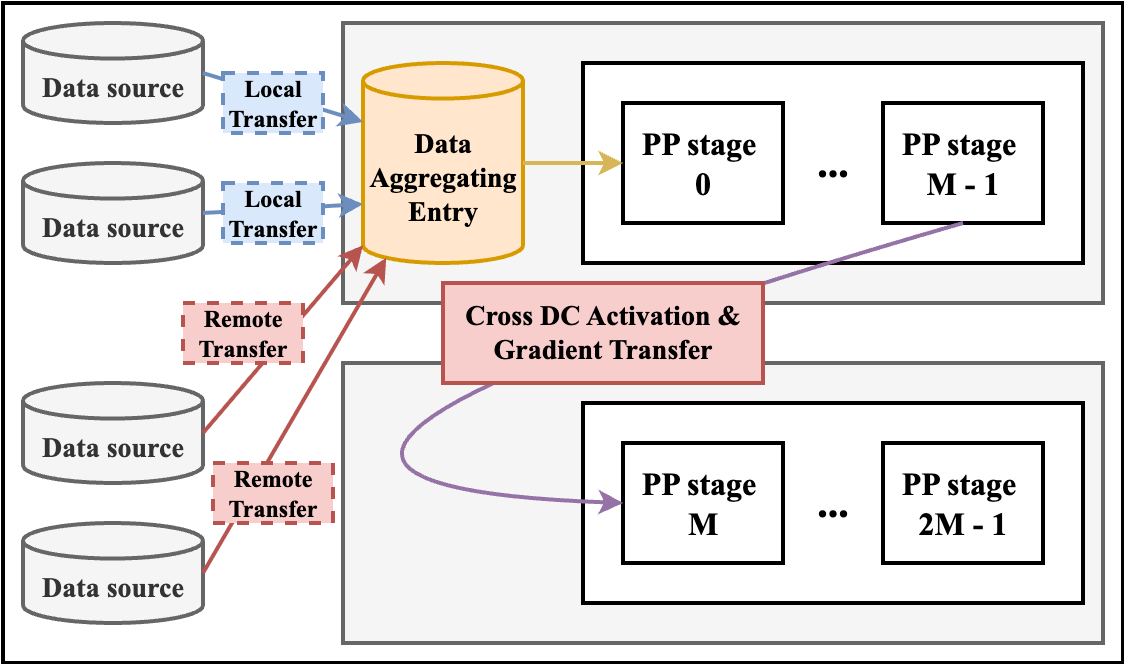
\includegraphics[width=0.96\columnwidth]{images/pp_across_dcs.png}
    \caption{Cross-DC pipeline parallelism. All training data must be aggregated at a single entry-point datacenter, creating severe ingress bottlenecks.}
    \label{fig:cross-dc-pp}
\end{figure}

\begin{figure}[ht]
    \centering
    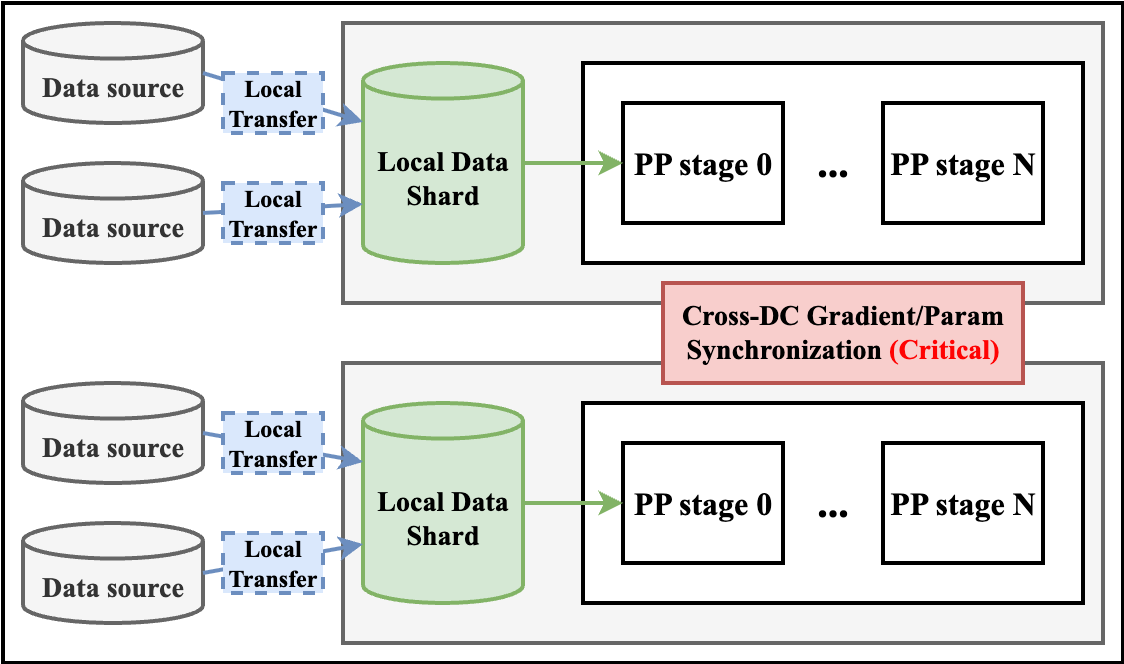
\includegraphics[width=0.96\columnwidth]{images/dp_across_dcs.png}
    \caption{Cross-DC data parallelism with intra-datacenter pipeline parallelism (our setting). Each datacenter processes local data and synchronizes only gradients across the WAN.}
    \label{fig:cross-dc-dp}
\end{figure}

\subsubsection{Parallelism Backbones Indicate a Fundamental Design Trade-off}

To scale training under these constraints, existing Cross-DC systems adopt different parallelism backbones that define how computation and communication are organized across datacenters. Pipeline-parallel–centric designs partition the model into sequential stages and stream micro-batches through the pipeline, enabling training of models that exceed the capacity of individual devices or clusters. Several Cross-DC systems\cite{DBLP:conf/usenix/ChenKHH25, DBLP:journals/corr/abs-2510-12064, DBLP:conf/hotnets/DengS00025} adopt pipeline parallelism as their primary backbone, leveraging its high compute efficiency under ideal communication conditions.

In contrast, data-parallel-centric designs replicate the model across datacenters and partition the dataset instead. Each datacenter performs forward and backward computation locally, while periodically synchronizing model updates across sites. This approach aligns naturally with data locality and minimizes cross-datacenter data movement during the main computation phase, at the cost of explicit synchronization.

\subsubsection{Synchronization and Communication Practices}

Independent of the chosen parallelism backbone, Cross-DC training systems differ in how they synchronize model updates across datacenters. Fully synchronous schemes enforce global barriers at every iteration, preserving strict optimization semantics but exposing WAN latency directly on the training critical path. Asynchronous schemes decouple computation from synchronization, allowing workers to proceed independently, but introduce gradient staleness and potential model divergence. Periodic or local synchronization strategies amortize communication cost by performing multiple local updates before synchronization, trading reduced communication frequency for increased optimization drift.

Collectively, prior work reveals a fundamental tension: synchronization is either frequent and expensive under WAN conditions, or relaxed in ways that perturb the optimization trajectory. This tension motivates a closer examination of how parallelism choices and synchronization interact in Cross-DC environments.

\subsection{Motivation}

\subsubsection{Rethinking Parallelism Choices in Cross-DC Training}
\label{ssb:rethink_parallelism}
Pipeline parallelism is widely regarded as compute-efficient when training is evaluated from a computation-only perspective. By overlapping forward and backward execution across stages, PP can achieve high device utilization under stable, low-latency communication. However, in Cross-DC settings, training efficiency is shaped not only by computation but also by data movement and network dynamics.

In PP-centric Cross-DC designs, training samples or activations must enter the pipeline and be propagated across stages that may span multiple datacenters. Pipeline execution enforces strict ordering constraints between stages, causing delays in cross-datacenter communication to directly stall downstream computation. As illustrated in Figure \ref{fig:cross-dc-pp}, data availability, pipeline progress, and WAN performance become tightly coupled: a slowdown or transient latency spike affecting a single stage can cascade through the pipeline and amplify end-to-end iteration time.

In contrast, data-parallel centric designs localize forward and backward computation within each datacenter. Data loading, preprocessing, and model execution proceed without reliance on WAN communication, and cross-datacenter interaction is confined to synchronization phases outside the main execution path (Figure \ref{fig:cross-dc-dp}). As a result, DP-centric designs are inherently more robust to network variability. 

Our theoretical proofs in the \ref{app:rethink_parallelism} reveal that in scenarios involving training large amounts of data across data centers, the throughput using cross-data center data parallelism is significantly higher than that of cross-data center pipeline parallelism. These observations motivate a hierarchical DP+PP architecture, in which data parallelism is used across data centers to ensure locality and robustness, while pipeline parallelism is employed within each data center to scale model capacity\cite{DBLP:journals/pvldb/KloudasRPM15}.

\subsubsection{Synchronization Becomes the Dominant Bottleneck}

% \begin{figure}[t]
%     \centering
%     \includegraphics[width=0.96\columnwidth]{example-image-duck}
%     \caption{Training flow in DP-based Cross-DC training.}
%     \label{fig:training_flow_dp_based}
% \end{figure}

While a DP+PP backbone addresses data locality and execution robustness, it exposes a new performance bottleneck: cross-datacenter synchronization. In DP-based Cross-DC training, each datacenter independently executes forward and backward passes on local data, but must synchronize model updates to maintain a consistent global model state. 

Under WAN conditions, synchronization latency is no longer negligible. A breakdown of iteration time under a DP+PP configuration (Figure \ref{fig:dppp_timebreakdown}) shows that synchronization in cross-DC scenario can account for a substantial fraction of total iteration time. Consequently, GPUs remain idle for a large fraction of time, waiting for synchronization to complete. 

\begin{figure}[ht]
    \centering
    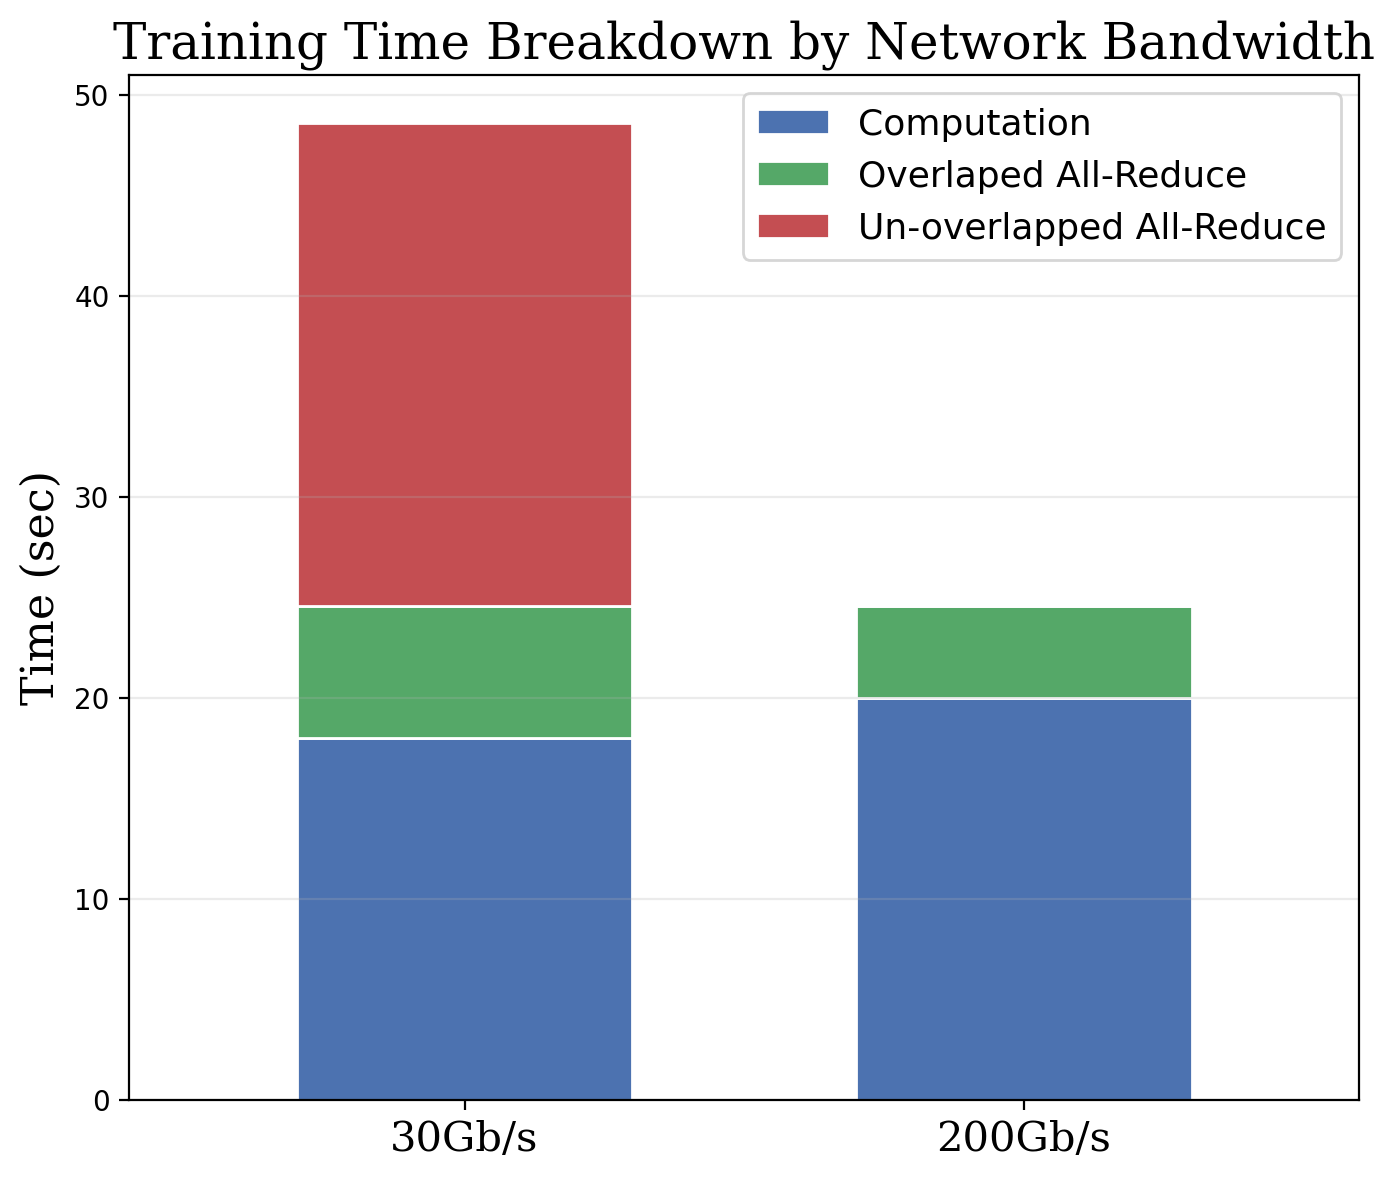
\includegraphics[width=0.96\columnwidth]{images/bar_time_by_network.png}
    \caption{Breakdown of computation and communication overhead per training step under a DP+PP configuration across and within datacenters.}
    \label{fig:dppp_timebreakdown}
\end{figure}



Importantly, existing communication overlap mechanisms in standard data-parallel frameworks\cite{DBLP:journals/pvldb/ZhaoGVLHXWSOSDB23, DBLP:journals/pvldb/LiZVSNLPSVDC20, DBLP:conf/sc/RajbhandariRRH20} only overlap gradient communication within a single backward pass. Under WAN-scale latency, the tail of the synchronization inevitably extends beyond the available computation, making end-of-step blocking unavoidable. Thus, while DP+PP mitigates data-movement inefficiencies, it shifts the primary performance bottleneck to synchronization.


\subsubsection{Decoupling Synchronization Without Sacrificing Optimization Semantics}
A natural response to the synchronization bottleneck is to adopt partially asynchronous methods such as Local-SGD\cite{stich2019local}. However, these schemes exhibit two principal limitations: unresolved performance bottlenecks and an increased risk of model drift during training.\cite{KarimireddyKMRS20, DBLP:conf/iclr/GuLHA23}

From a performance perspective, Local-SGD primarily reduces the frequency of cross-datacenter synchronization rather than eliminating the communication costs inherent to distributed optimization. Periodic global aggregation remains unavoidable. The consequence is sustained GPU idle time.

From an optimization/precision perspective, increasing the number of local steps elevates the risk of model drift. Gradients computed on these stale local replicas introduce systematic bias; this bias can slow convergence and degrade practical generalization performance.

These observations suggest that merely weakening synchronization is insufficient. Conversely, some fully asynchronous schemes\cite{DBLP:journals/corr/abs-2407-07852, DBLP:journals/corr/abs-2501-18512} eliminate compute bubbles but incur severe parameter staleness that is difficult to correct. An effective cross-datacenter training system therefore needs to decouple synchronization from the training critical path while preserving convergence robustness comparable to fully synchronous optimization, rather than relying on strict equivalence of update sequences.


This insight motivates the design of POLAR-SGD.


    % \section{Motivation}
    % \input{section/motivation}

    \section{\sysname Design}
    \label{sec:design}

In this section, we present POLAR-SGD (Predictive Overlap in Local SGD with Adaptive Redundancy), a novel approach designed to address the communication bottleneck in DP+PP hybrid parallel training. The core principle is to transform blocking gradient synchronization into a pipelined communication process that overlaps with computation, while maintaining model convergence stability through a predictive error-correction mechanism.

\subsection{Notation}

We first introduce the key notation used throughout this section. Table~\ref{tab:notation} summarizes the symbols and variables employed in our algorithms.

\begin{table}[ht]
\centering
\caption{Notation and terminology used in POLAR-SGD}
\label{tab:notation}
\begin{tabular}{ll}
\hline
\textbf{Symbol} & \textbf{Description} \\
\hline
$M$ 
& Number of micro-batches per mini-batch \\
$m$
& Micro-batch index \\
$t$ 
& Global iteration index \\
$r$ 
& Worker index (rank) within a DP group \\
$g_{r,t,m}$ 
& Gradient of worker $r$ at iteration $t$ \\
& for micro-batch $m$ \\
$g_{r,t}^{(\tau)}$      
& Prefix accumulated gradient on worker $r$ \\
& up to micro-batch $\tau$ \\
$g_{r,t}^{(M)}$         
& Full accumulated gradient on worker $r$ up \\
& to micro-batch $M$ \\
$g_{\mathrm{pred},r,t}$ 
& Predicted (scaled) gradient sent to \\
& All-Reduce at iteration $t$ \\
$g_{\mathrm{sync},t}$ 
& Synchronized gradient from All-Reduce \\
& (mean across DP workers) \\
$e_{r,t}$ 
& Error buffer on worker $r$ at iteration $t$ \\
$s_{r,t}$ 
& Send buffer for communication at iteration $t$ \\
$h_t$ 
& Communication handle at iteration $t$ \\
$w_t$ 
& Model weights at global iteration $t$ \\
$\eta$ 
& Learning rate \\
$N$ 
& DP group size (number of workers partic- \\
& ipated in All-Reduce) \\
$T$ 
& Number of global iterations \\
$\tau$ 
& Communication cutoff micro-batch index \\
\hline
\end{tabular}
\end{table}

\begin{figure*}[t]
    \centering
    
\includegraphics[width=0.96\textwidth]{images/polar-pp-timeline.png}
    \caption{
        \textbf{Execution timeline comparison under DP+PP.} We illustrate one global iteration with $M{=}8$ micro-batches, DP size $=2$, and PP size $=4$. Each row labeled as \textit{Rank $x/x{+}4$} represents the same pipeline stage replicated across the two data-parallel ranks (e.g., Rank $0/4$ denotes stage 0 on the two DP replicas).
        \textbf{Top: Baseline (PyTorch/Megatron).} Gradient synchronization is performed in a blocking manner near the end of the mini-batch, forming a long All-Reduce tail (purple) after most backward computations (white) have finished, which leaves accelerators under-utilized.
        \textbf{Bottom: POLAR-SGD.} We launch non-blocking All-Reduce after the prefix micro-batches up to cutoff $\tau$ are accumulated, and offload the collective to a dedicated communication stream, thereby overlapping All-Reduce (purple) with subsequent backward computations (white) and shrinking the iteration tail.
    }
    \label{fig:overview}
\end{figure*}

\subsection{Overview of POLAR-SGD}

Figure~\ref{fig:overview} compares the execution timelines of a standard DP+PP training loop and our POLAR-SGD design. The example uses $M{=}8$ micro-batches per mini-batch, DP size $=2$, and PP size $=4$ (i.e., 8 global ranks in total). In the figure, each row labeled as \textit{Rank $x/x{+}4$} aggregates the behavior of the same pipeline stage across the two data-parallel replicas; for instance, \textit{Rank $0/4$} corresponds to pipeline stage 0 on the two DP ranks.

\textbf{Baseline DP+PP suffers from a synchronization tail.}
As shown in Figure~\ref{fig:overview}(top), pipeline parallelism interleaves forward (red) and backward (white) computations across stages and micro-batches, but data-parallel gradient synchronization is typically deferred until the end of the mini-batch after all $M$ micro-batches have completed backward. Consequently, a large blocking All-Reduce phase (purple) appears near the end of the iteration, leading to significant accelerator idle time and reduced throughput.

\textbf{POLAR-SGD eliminates the tail via prefix-based early synchronization.}
Figure~\ref{fig:overview}(bottom) illustrates our key idea: we trigger \emph{exactly one} asynchronous All-Reduce earlier within the iteration, after only a prefix of micro-batches has finished backward. While the collective runs in the background, the main compute stream continues executing backward for the remaining micro-batches. The remaining $(M-\tau)$ micro-batches are incorporated through an error-feedback residual carried to the next iteration. Thus, POLAR-SGD does not discard gradient information; it postpones the utilization of a portion of the mini-batch to enable communication--computation overlap with stable optimization behavior.

\subsection{Pipelined Gradient Communication}

\begin{algorithm}[tb]
  \caption{POLAR-SGD: Prefix-based pipelined gradient communication (one All-Reduce per iteration)}
  \label{alg:communication}
  \begin{algorithmic}
    \STATE {\bfseries Global variables:} accumulated gradient $g_a$, prefix snapshot $g^{(\tau)}$, communication handle $h$
    \STATE {\bfseries Procedure:} OnBackwardMicroBatch$(t,m,g_{r,t,m})$
    \STATE $g_a \leftarrow g_a + g_{r,t,m}$  \COMMENT{PP gradient accumulation}
    \IF{$m == \tau$}
      \STATE $g^{(\tau)} \leftarrow g_a$  \COMMENT{snapshot prefix gradient}
      \STATE (build send buffer $s_{r,t}$ as in Algorithm~\ref{alg:error_feedback})
      \STATE $h \leftarrow$ AsyncAllReduce$(s_{r,t})$
    \ENDIF
    \IF{$m == M$}
      \STATE \textbf{wait}($h$); \hfill \COMMENT{obtain $g_{\mathrm{sync},t}$ (mean across DP workers)}
      \STATE OptimizerStep($g_{\mathrm{sync},t}$)
      \STATE $g_a \leftarrow 0$
      \STATE $h \leftarrow NULL$
    \ENDIF
  \end{algorithmic}
\end{algorithm}

% In standard DP+PP, a mini-batch is divided into $M$ micro-batches. For worker $r$ in a DP group, local gradients are accumulated as
% \begin{equation}
%     g_{r,t}^{(M)} = \sum_{m=1}^{M} g_{r,t,m},
% \end{equation}
% and a blocking All-Reduce is performed after all micro-batches complete.

After the backward pass of each micro-batch $m$ finishes, we accumulate its gradient into a running buffer. When $m=\tau$, we launch a non-blocking All-Reduce on a communication buffer built from the current prefix-accumulated gradient. The \texttt{GradientUpdateJudge} function returns true only at the end of the mini-batch ($m=M$), where we wait for the asynchronous communication to complete and then apply the optimizer step.

\paragraph{Choosing the cutoff $\tau$.}
Let $T_{\mathrm{ar}}$ be the estimated All-Reduce latency (mean) for the communicated gradient tensor, and let $T_{\mathrm{comp}}(\tau)$ denote the remaining computation time after launching communication at micro-batch $\tau$ within the same iteration. We select the earliest cutoff that can fully hide communication:
\begin{equation}
\tau^* \triangleq \min \left\{\tau \in \{1,\ldots,M\}:\; T_{\mathrm{comp}}(\tau) \ge T_{\mathrm{ar}}\right\},
\label{eq:tau_rule}
\end{equation}
% and fall back to $\tau^*=M$ when the inequality is not satisfied for any $\tau$. 
In practice, $T_{\mathrm{ar}}$ and $T_{\mathrm{comp}}(\tau)$ can be obtained from online profiling with a sliding-window average. Intuitively, smaller $\tau$ yields more overlap but increases the reliance on error feedback; larger $\tau$ reduces approximation and recovers the baseline behavior.

\subsection{Predictive Error Correction}

Launching All-Reduce early means that the parameter update is only based on a \emph{prefix} gradient.

POLAR-SGD addresses this by forming a full-batch-scale \emph{predicted} gradient at $m=\tau$ and maintaining an error buffer that captures the mismatch between the prediction and the full accumulation.

\paragraph{Prefix and full gradients.}
On worker $r$ at iteration $t$, define the prefix accumulated gradient and the full accumulated gradient as
\begin{equation}
g_{r,t}^{(\tau)} \triangleq \sum_{m=1}^{\tau} g_{r,t,m},
\qquad
g_{r,t}^{(M)} \triangleq \sum_{m=1}^{M} g_{r,t,m}.
\end{equation}
At $m=\tau$, $g_a$ equals $g_{r,t}^{(\tau)}$; after $m=M$, $g_a$ equals $g_{r,t}^{(M)}$.

\paragraph{Predicted gradient and error update (full-batch scale).}
At the cutoff point $m=\tau$, we form the send buffer
\begin{equation}
s_{r,t} = \frac{M}{\tau}\left(g_{r,t}^{(\tau)} + e_{r,t}\right),
\label{eq:sendbuf}
\end{equation}
and record the predicted (pre-reduction) gradient as
\begin{equation}
g_{\mathrm{pred},r,t} \triangleq s_{r,t}.
\end{equation}
We then perform a non-blocking All-Reduce \emph{mean} over $s_{r,t}$ across the DP group and obtain the synchronized gradient
\begin{equation}
g_{\mathrm{sync},t} = \frac{1}{N}\sum_{r=1}^{N} g_{\mathrm{pred},r,t}.
\end{equation}

After finishing all $M$ micro-batches, we update the error buffer by the mismatch between the \emph{full} accumulated gradient and the predicted gradient:
\begin{equation}
e_{r,t+1} = g_{r,t}^{(M)} - g_{\mathrm{pred},r,t}.
\label{eq:error_update}
\end{equation}
This residual contains the information from the remaining $(M-\tau)$ micro-batches (and any prediction error) and is injected into the next iteration through Eq.~\eqref{eq:sendbuf}. Thus, POLAR-SGD does not discard gradients from later micro-batches; it defers their effect via a controlled error-feedback pathway.

% 下面这些放到附录里
% \paragraph{Averaged conservation property.}
% Let $\bar g_t^{(\tau)}=\frac{1}{N}\sum_r g_{r,t}^{(\tau)}$, $\bar g_t^{(M)}=\frac{1}{N}\sum_r g_{r,t}^{(M)}$, and $\bar e_t=\frac{1}{N}\sum_r e_{r,t}$. Averaging Eq.~\eqref{eq:error_update} across workers yields
% \begin{equation}
% g_{\mathrm{sync},t} + \bar e_{t+1} = \bar g_t^{(M)},
% \label{eq:conservation}
% \end{equation}
% which shows that the synchronized update direction plus the averaged residual exactly recovers the full-batch accumulated gradient for that iteration.

\begin{algorithm}[tb]
  \caption{POLAR-SGD: Error feedback with prefix scaling}
  \label{alg:error_feedback}
  \begin{algorithmic}
    \STATE {\bfseries Global variables:} error buffer $e_{r,t}$, predicted gradient $g_{\mathrm{pred},r,t}$, cutoff $\tau$, $M$
    \STATE Initialize: $e_{r,0} \leftarrow 0$
    \STATE {\bfseries Procedure:} {BuildSendBufferAtCutoff}$(t, g_{r,t}^{(\tau)})$
    \STATE $s_{r,t} \leftarrow \frac{M}{\tau}\left(g_{r,t}^{(\tau)} + e_{r,t}\right)$
    \STATE $g_{\mathrm{pred},r,t} \leftarrow s_{r,t}$
    
    \STATE \textbf{return} $s_{r,t}$ \COMMENT{passed to AsyncAllReduce in Algorithm~\ref{alg:communication}}
    \STATE {\bfseries Procedure:} UpdateError $(t, g_{r,t}^{(M)})$
    \STATE $e_{r,t+1} \leftarrow g_{r,t}^{(M)} - g_{\mathrm{pred},r,t}$
  \end{algorithmic}
\end{algorithm}

\subsection{Convergence Analysis}

% We provide a convergence analysis showing that POLAR-SGD retains the same \emph{asymptotic} convergence behavior as synchronous SGD, up to an additional term controlled by the error-feedback residual.

% \subsubsection{Assumptions}

% We make the following standard assumptions in stochastic optimization:

% \begin{assumption}[L-Smoothness]
% \label{assump:smooth}
% The loss function $f(w)$ is $L$-smooth, i.e., for all $w, w'$:
% \begin{equation}
%     \|\nabla f(w) - \nabla f(w')\| \leq L \|w - w'\|.
% \end{equation}
% \end{assumption}

% \begin{assumption}[Unbiased Gradient]
% \label{assump:unbiased}
% For each worker $r$ and micro-batch $m$, the stochastic gradient is unbiased:
% \begin{equation}
% \mathbb{E}\left[g_{r,t,m}\mid w_t\right] = \nabla f(w_t).
% \end{equation}
% \end{assumption}

% \begin{assumption}[Bounded Variance]
% \label{assump:variance}
% The variance of stochastic gradients is bounded:
% \begin{equation}
% \mathbb{E}\left[\|g_{r,t,m} - \nabla f(w_t)\|^2 \mid w_t\right] \le \sigma^2.
% \end{equation}
% \end{assumption}

% \noindent
% % \textbf{Remark.} Our analysis focuses on the DP synchronization effect introduced by prefix-based communication. The pipeline execution order does not change the definition of per-micro-batch stochastic gradients; gradients are accumulated normally over $M$ micro-batches within each iteration.

% \subsubsection{Main Convergence Theorem}

% \begin{theorem}[Convergence of POLAR-SGD (mean All-Reduce with error feedback)]
% \label{thm:convergence}
% Under Assumptions~\ref{assump:smooth}--\ref{assump:variance}, with learning rate $\eta \leq \frac{1}{2L}$, after $T$ global iterations, POLAR-SGD satisfies
% \begin{equation}
% \begin{aligned}
% \frac{1}{T}\sum_{t=0}^{T-1}\mathbb{E}\left[\|\nabla f(w_t)\|^2\right]
% \le\;&
% \frac{2\big(f(w_0)-f^*\big)}{\eta T}
% + \frac{L\eta\sigma^2}{N}
% \\
% &+ \frac{L\eta}{T}\sum_{t=0}^{T-1}\mathbb{E}\left[\|\bar e_t\|^2\right],
% \end{aligned}
% \label{eq:main_bound}
% \end{equation}
% where $f^*=\inf_w f(w)$ and $\bar e_t=\frac{1}{N}\sum_{r=1}^N e_{r,t}$ is the averaged error buffer.
% \end{theorem}

% \noindent
% The complete proof is provided in Appendix~\ref{app:proof}. In brief, the proof follows the standard smoothness-based descent analysis for SGD, with the update direction $g_{\mathrm{sync},t}$ and the conservation property in Eq.~\eqref{eq:conservation} used to relate $g_{\mathrm{sync},t}$ to the full accumulated gradient $\bar g_t^{(M)}$ plus a residual term $\bar e_{t+1}$.

% \subsubsection{Key Insights}

% Theorem~\ref{thm:convergence} implies the following:

% \begin{enumerate}
%     \item \textbf{Asymptotic convergence rate.}
%     When the averaged residual $\bar e_t$ remains bounded (which is empirically observed and can be encouraged by choosing $\tau$ via Eq.~\eqref{eq:tau_rule}), POLAR-SGD achieves the same $O(1/\sqrt{T})$-type asymptotic behavior as synchronous SGD, up to an additional constant term controlled by $\mathbb{E}\|\bar e_t\|^2$.

%     \item \textbf{No gradient information is discarded.}
%     Eq.~\eqref{eq:conservation} shows that the synchronized update direction and the averaged residual exactly decompose the full accumulated gradient $\bar g_t^{(M)}$. Thus, gradients from later micro-batches are not dropped; their effect is deferred through the error buffer.

%     \item \textbf{Variance reduction from data parallelism.}
%     With mean All-Reduce over $N$ workers, the stochastic gradient variance scales as $\sigma^2/N$, matching standard DP training (captured by the second term on the RHS of Eq.~\eqref{eq:main_bound}).
% \end{enumerate}

% This analysis confirms that POLAR-SGD achieves communication--computation overlap while retaining stable optimization behavior, with the approximation explicitly captured by the residual term.

Under standard assumptions (L-smoothness, unbiased gradient, bounded variance), we prove POLAR-SGD achieves the same asymptotic convergence rate as synchronous SGD (see \ref{app:proof} for full proof). The key theorem shows the average gradient norm bound only includes an additional constant term controlled by the error buffer, confirming stable optimization behavior.

    % % \section{Implementation}
    % % \label{implementation}

    % \label{sec:implementation}

We implement POLAR-SGD as a lightweight extension to PyTorch's \texttt{DistributedDataParallel} (DDP) module.  Our implementation is fully compatible with existing DP+PP training pipelines and requires minimal code changes to deploy.

\subsection{Architecture Overview}

Figure~\ref{fig:implementation_arch} illustrates the system architecture.  POLAR-SGD intercepts PyTorch's gradient computation events through backward hooks, manages asynchronous All-Reduce operations via a communication handle queue, and maintains per-parameter error buffers for gradient correction.  The core logic is encapsulated in a custom DDP wrapper that transparently implements Algorithms~\ref{alg:communication} and~\ref{alg:error_feedback}.

\begin{figure}[t]
    \centering
    \includegraphics[width=\columnwidth]{example-image-duck}
    \caption{POLAR-SGD system architecture. The implementation intercepts gradient hooks, manages asynchronous communication, and maintains error buffers without requiring changes to the training loop.}
    \label{fig:implementation_arch}
\end{figure}

\textbf{Key implementation choices. } We leverage three PyTorch primitives:  (1) \texttt{register\_comm\_hook} to intercept gradient readiness, (2) \texttt{torch.distributed.iallreduce} for non-blocking communication, and (3) gradient buffers for error accumulation. The backward hook is triggered automatically after each micro-batch's gradient computation, initiating the compensated All-Reduce ($s = g_a + e$) and storing the communication handle for later synchronization.  When a parameter update is triggered, we wait for the pending All-Reduce, compute the new error ($e = g_{sync} - g_{pred}$), and proceed with the optimizer step.

\subsection{Integration and Compatibility}

\textbf{Drop-in replacement for DDP.} Migrating from standard PyTorch DDP to POLAR-SGD requires only replacing the model wrapper. No other changes to the training script, optimizer, or data loader are needed. The training loop remains identical to standard DDP training.

\textbf{Pipeline parallelism integration.} POLAR-SGD operates at the data-parallel dimension and is orthogonal to pipeline parallelism. It integrates with existing pipeline-parallel training frameworks without modifying PP schedules (1F1B, interleaved 1F1B, etc.). We validated compatibility across multiple PP implementations.

\textbf{Mixed precision and gradient accumulation.} Our implementation supports FP16/BF16 mixed precision training via PyTorch's \texttt{autocast}, maintaining error buffers in the same precision as gradients.  Gradient accumulation is naturally supported—errors accumulate across micro-batches and are corrected at mini-batch boundaries. 

\subsection{Overhead and Tuning}

\textbf{Memory and computation costs.} POLAR-SGD introduces minimal overhead:  one gradient-sized error buffer per parameter (e.g., 14 GB for a 7B model in FP16) and two element-wise additions per micro-batch ($<0.1\%$ computational overhead). Communication volume is identical to standard DDP. 

\textbf{Configuration parameters.} Two parameters control the trade-off between overlap and staleness: 
\begin{itemize}
    \item \texttt{comm\_freq}: How often to trigger All-Reduce (every $K$ micro-batches). Higher values reduce communication frequency but may limit overlap.
    \item \texttt{accum\_steps}: When to perform parameter updates (mini-batch size in micro-batches). Identical to standard gradient accumulation.
\end{itemize}
In our experiments (Section~\ref{sec:setup}), we find that \texttt{comm\_freq=2--4} provides optimal performance for Cross-DC scenarios with 20 Gb/s bandwidth and 50 ms latency.

\textbf{System requirements.} POLAR-SGD requires PyTorch 1.13+ and a communication backend supporting non-blocking operations (NCCL for GPUs, Gloo for CPUs). All workers in a DP group must use identical \texttt{comm\_freq} and \texttt{accum\_steps}.

Our implementation is available as an open-source package at \url{https://github.com/anonymous/polar-sgd}, including integration examples and documentation.    

    \section{Evaluation}
    \label{evaluation}

    % Evaluation
    \label{sec:evaluation}

In this section, we conduct a comprehensive evaluation of POLAR-SGD under a realistic cross-datacenter (Cross-DC) training setting. 
% Our experiments are designed to answer the following questions:
% \begin{enumerate}
%     \item How much end-to-end training efficiency can POLAR-SGD deliver compared to a standard DP+PP baseline under WAN-like network constraints?
%     \item Does POLAR-SGD remain effective and robust in a multi-node, multi-GPU environment without relying on unrealistic hardware assumptions?
%     \item Does the throughput gain come at the expense of convergence behavior or final model quality?
%     \item Is a stabilization mechanism (e.g., error-correction) necessary beyond merely pipelining or relaxing synchronization?
% \end{enumerate}

\subsection{Experimental Setup}
\label{sec:setup}

Table~\ref{tab:setup} summarizes our experimental configuration. We compare POLAR-SGD against a standard implementation, denoted as \textbf{Baseline DDP (Standard DP+PP)}. This baseline employs a 1F1B pipeline schedule and performs a blocking All-Reduce to synchronize gradients at the end of each mini-batch. Under WAN-like Cross-DC conditions, such barriered synchronization typically induces substantial stalls and reduces effective GPU utilization.

In addition, we include a representative relaxed synchronization baseline, \textbf{LSGD ($k=4$)}, to highlight how delayed/local synchronization can alter training dynamics.

\subsection{Main Results}

We report end-to-end throughput in tokens/s in Table~\ref{tab:throughput}. For POLAR-SGD, we additionally report the normalized speedup over the Baseline DDP. 

\begin{table}[t]
    \caption{Experimental setup.}
    \label{tab:setup}
    \centering
    \begin{tabular}{@{}ll@{}}
        \toprule
        \textbf{Component} & \textbf{Specification} \\
        \midrule
        Model & LLaMA-2 7B \\
        Dataset & WikiText-103 \\
        Hardware & 32$\times$ NVIDIA A100 (40GB) GPUs \\
                 & across 4 nodes \\
        Network & Bandwidth: 30 Gb/s; RTT latency: 50 ms \\
        Parallelism & Hybrid DP+PP (PP=8, DP=4); \\
                    & batch=256; microbatch=32 \\
        Software & PyTorch 2.5; NCCL 2.23; CUDA 12.1 \\
        Metrics & Throughput (tokens/s), training loss \\
        \bottomrule
    \end{tabular}
\end{table}

\begin{table}[t]
    \caption{End-to-end throughput under Cross-DC network constraints.}
    \label{tab:throughput}
    \centering
    \begin{tabular}{@{}lcc@{}}
        \toprule
        \textbf{Method} & \textbf{Throughput (tokens/s)} & \textbf{Speedup} \\
        \midrule
        DDP+1F1B & 5,350 & 1.00$\times$ \\
        LSGD ($k=4$) & 9,433 & 1.76$\times$ \\
        POLAR-SGD & 10,016 & 1.87$\times$ \\
        \bottomrule
    \end{tabular}
\end{table}

\begin{figure}[t]
    \centering
    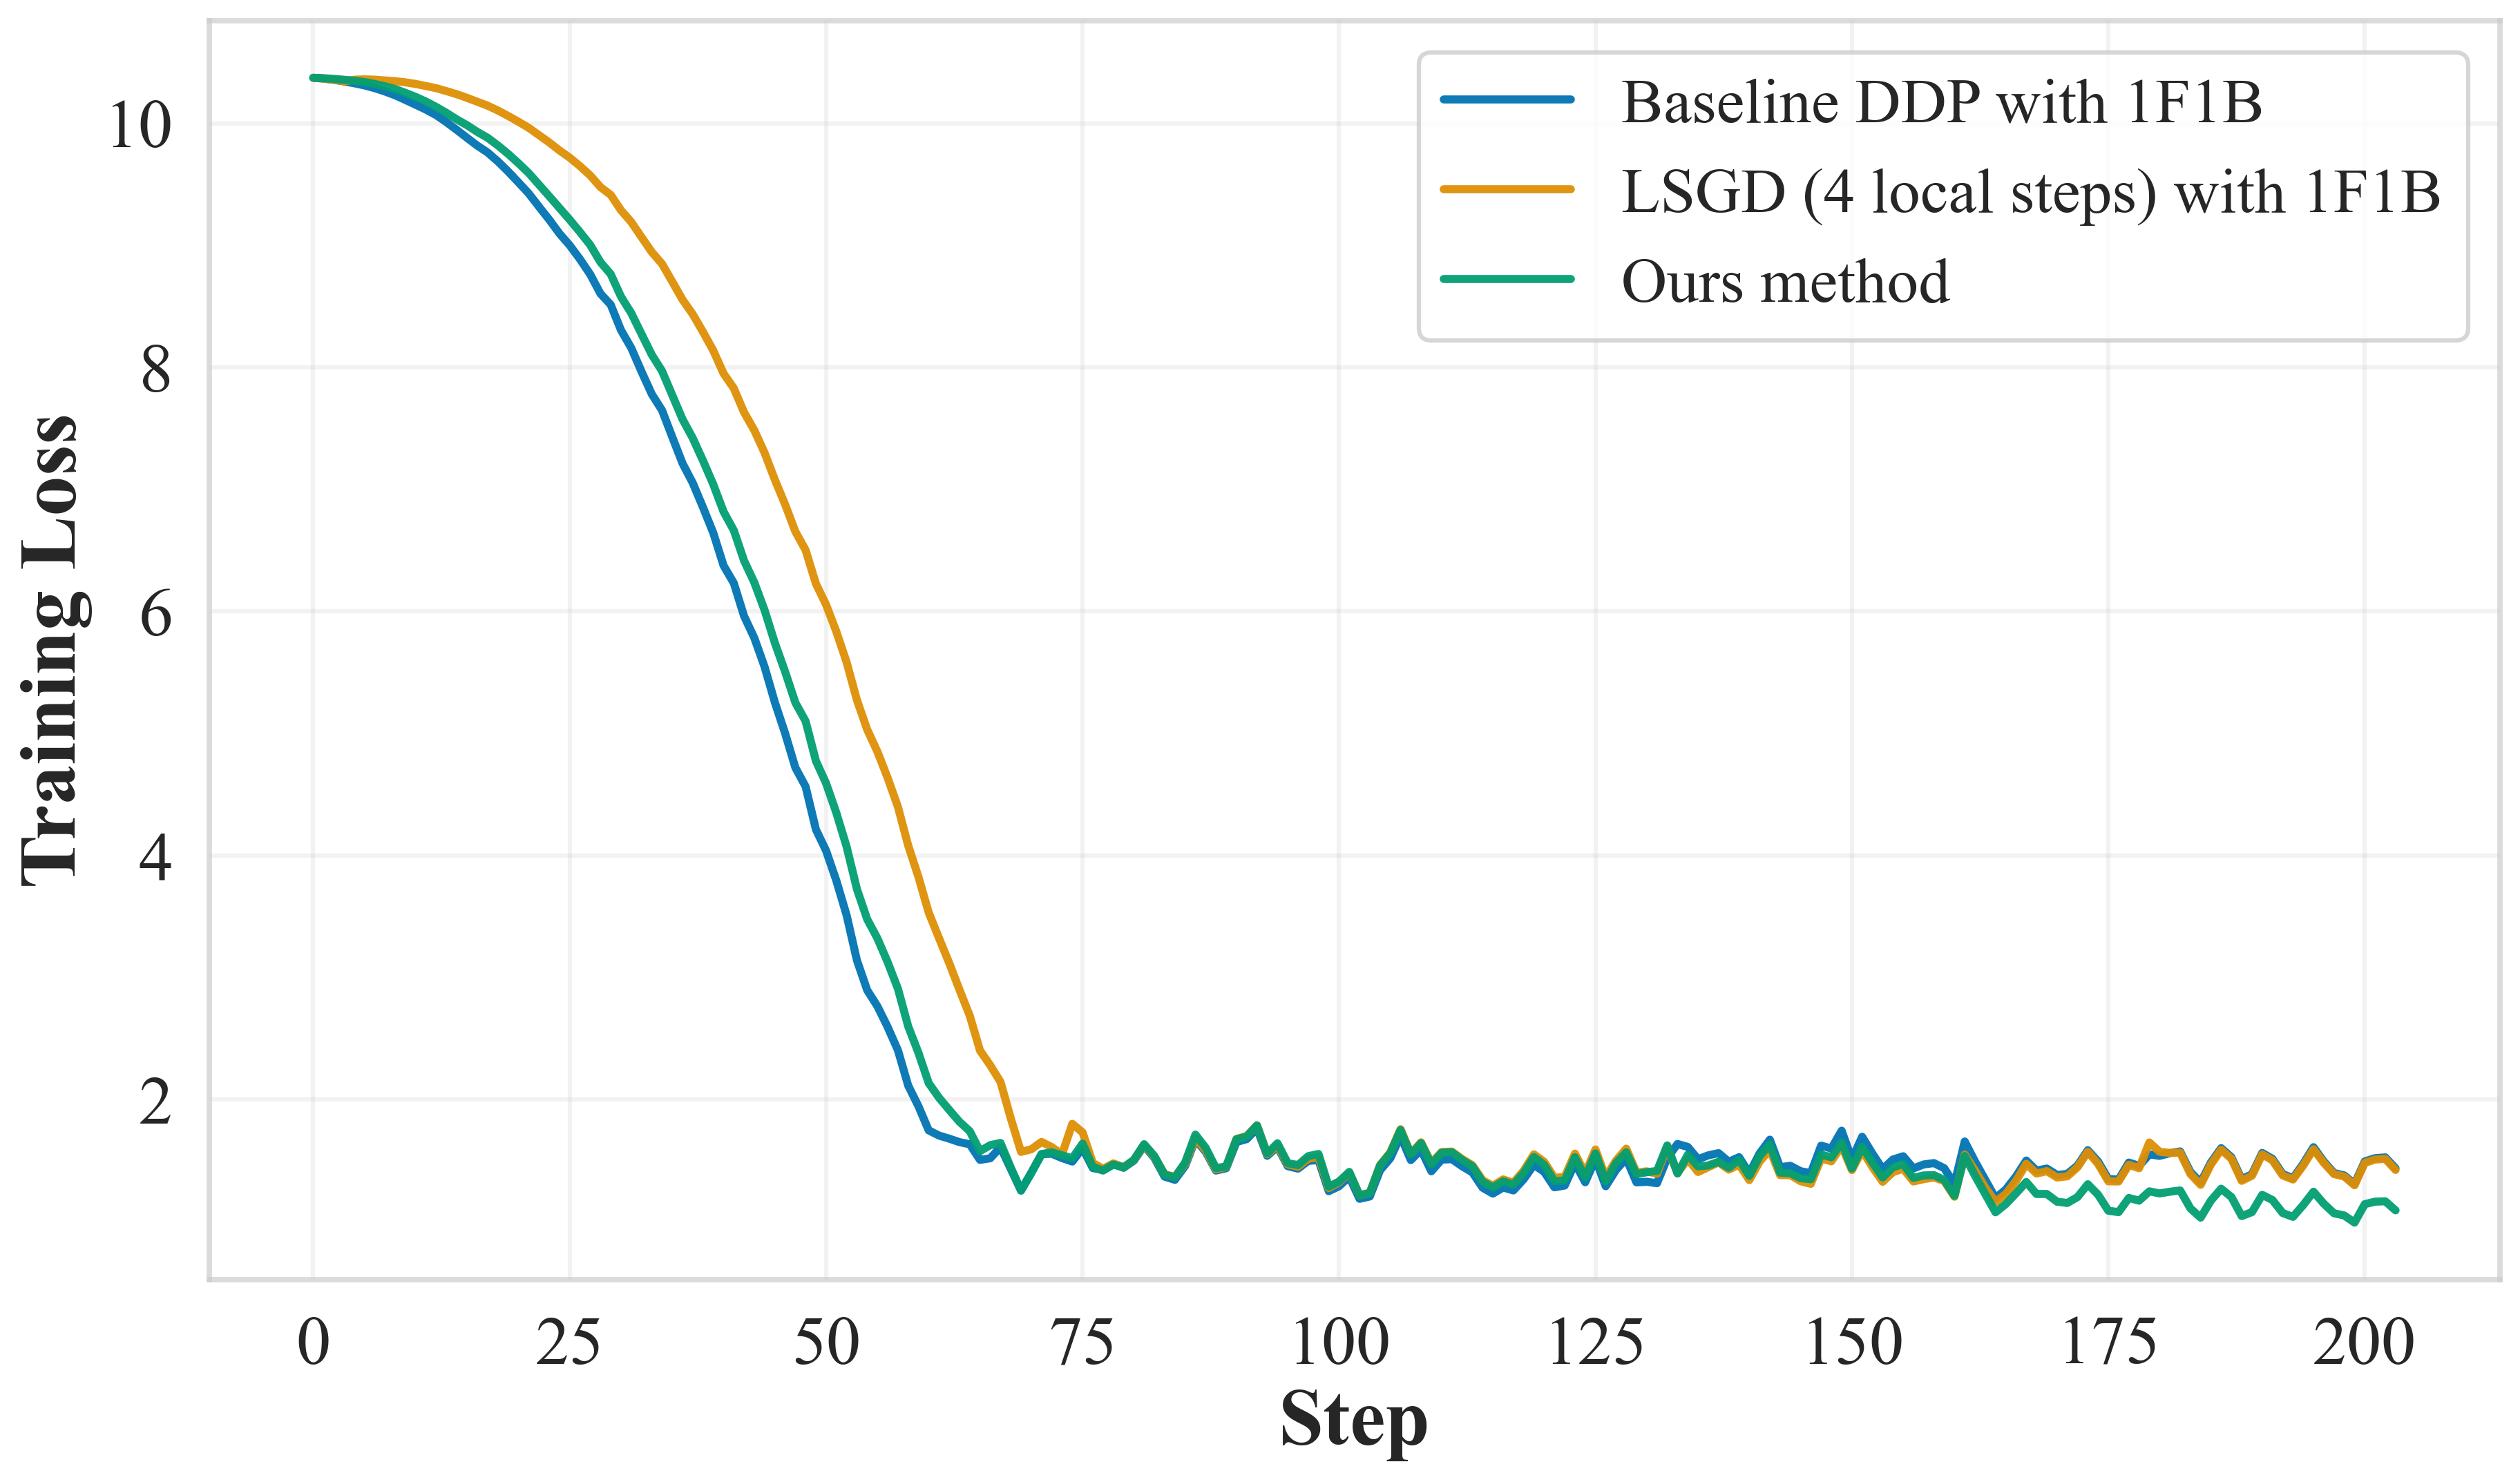
\includegraphics[width=\columnwidth]{images/json_curves_by_steps.png}
    \caption{Training loss versus steps on WikiText-103 (smoothed over a common step range). POLAR-SGD closely tracks the Baseline DDP, while LSGD shows a mild mid-to-late stage deviation, indicating that POLAR-SGD better preserves step-wise convergence stability under Cross-DC constraints.}
    \label{fig:loss_comparison}
\end{figure}

\begin{figure}[h]
    \centering
    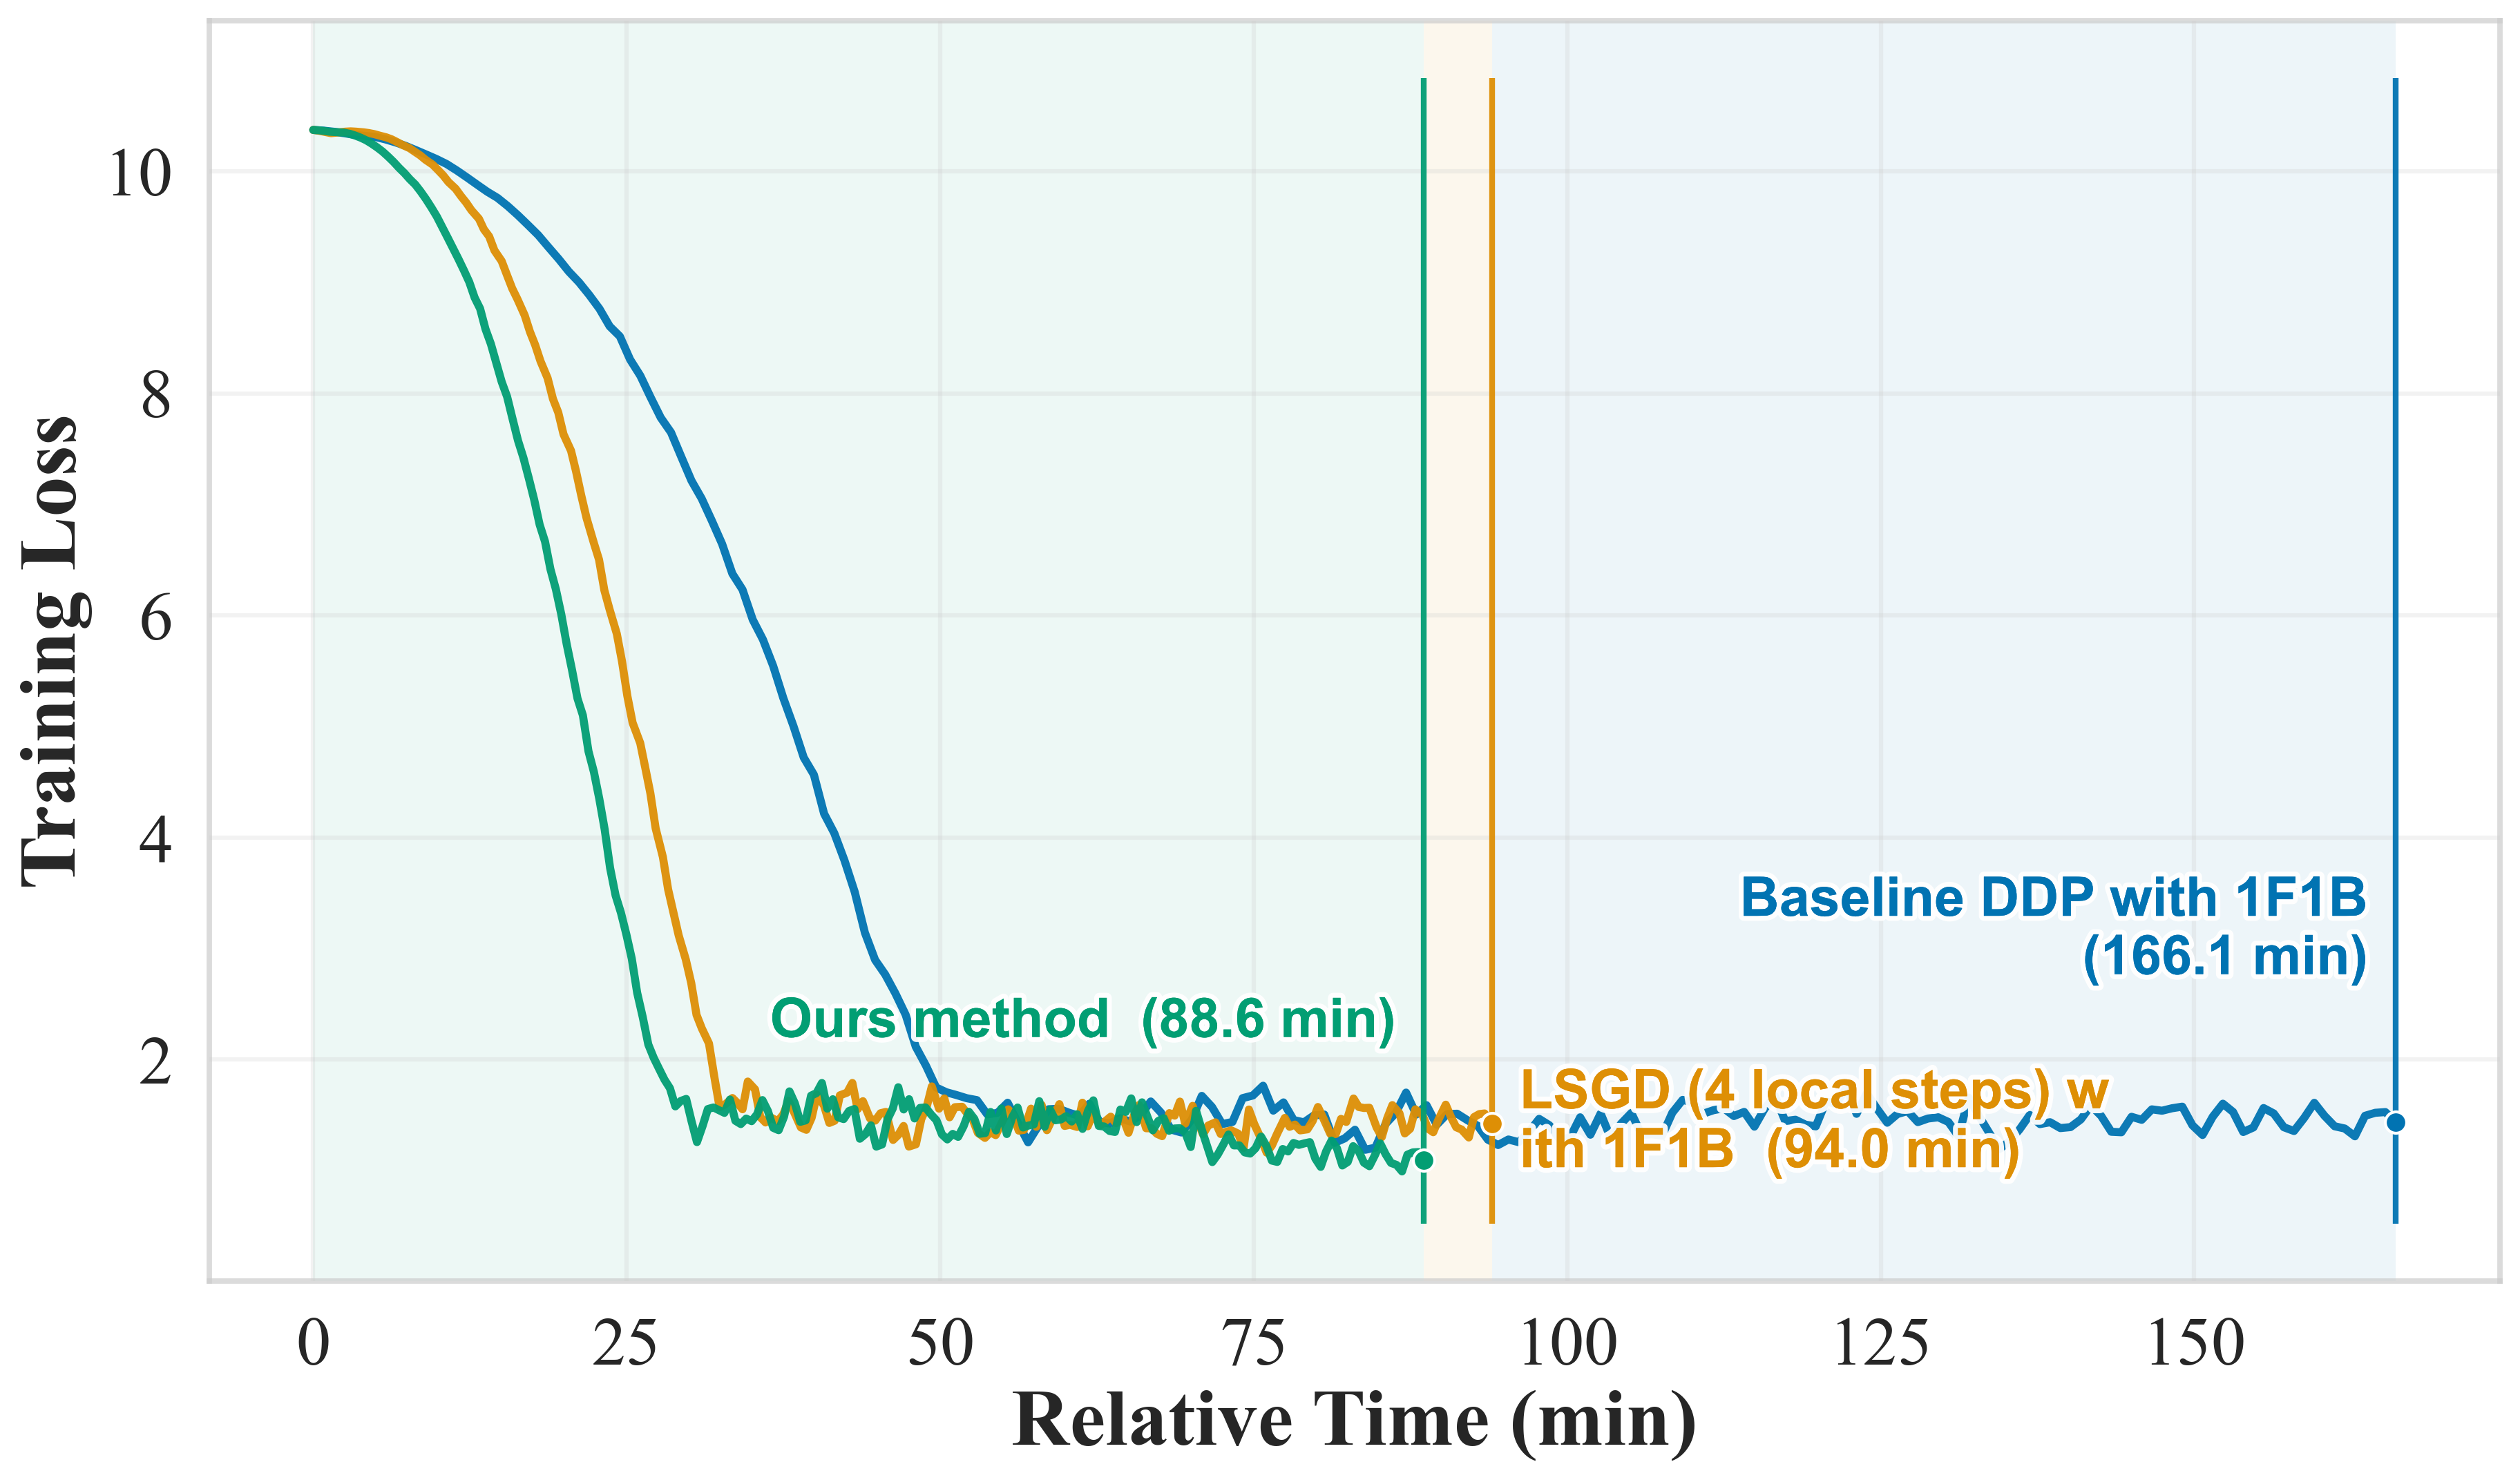
\includegraphics[width=\columnwidth]{images/json_curves_by_time.png}
    \caption{Training loss versus wall-clock time on WikiText-103 (smoothed). POLAR-SGD reaches the low-loss regime substantially earlier than the Baseline DDP, demonstrating improved time-to-target under Cross-DC network constraints.}
    \label{fig:loss_e2e_comparison}
\end{figure}

\paragraph{Convergence comparison by steps.}
Figure~\ref{fig:loss_comparison} reports the smoothed loss curves aligned by training steps over a common range. All methods exhibit a consistent overall trend: the loss decreases steadily and reaches a plateau after roughly 200 steps. Importantly, POLAR-SGD tracks the Baseline DDP closely across most of training, indicating that the proposed approach preserves stable optimization behavior despite introducing more aggressive communication/synchronization strategies. 

\paragraph{End-to-end convergence comparison by wall-clock time.}xs
The advantage of POLAR-SGD is more pronounced when comparing convergence as a function of wall-clock time. As shown in Figure~\ref{fig:loss_e2e_comparison}, POLAR-SGD reduces the loss substantially faster than the Baseline DDP under the same relative time budget. 
%Concretely, the baseline requires significantly longer time to reach a loss level comparable to POLAR-SGD, whereas POLAR-SGD enters the low-loss plateau much earlier. These results demonstrate that POLAR-SGD primarily improves \textbf{time-to-target}: even when step-wise convergence is similar, the reduced per-step overhead yields markedly better end-to-end training efficiency.

Taken together, Figures~\ref{fig:loss_comparison} and~\ref{fig:loss_e2e_comparison} support two conclusions. First, \textbf{convergence stability} is preserved: when aligned by steps, POLAR-SGD closely matches the baseline, showing no signs of instability or divergence. Second, \textbf{model quality is not sacrificed for throughput}: POLAR-SGD achieves comparable training loss while substantially reducing wall-clock time.


\subsection{Ablation Study}
\label{sec:ablation}

% NOTE: keep the ablation figure omitted until data is ready to avoid empty floats.
\begin{figure}[t]
    \centering
    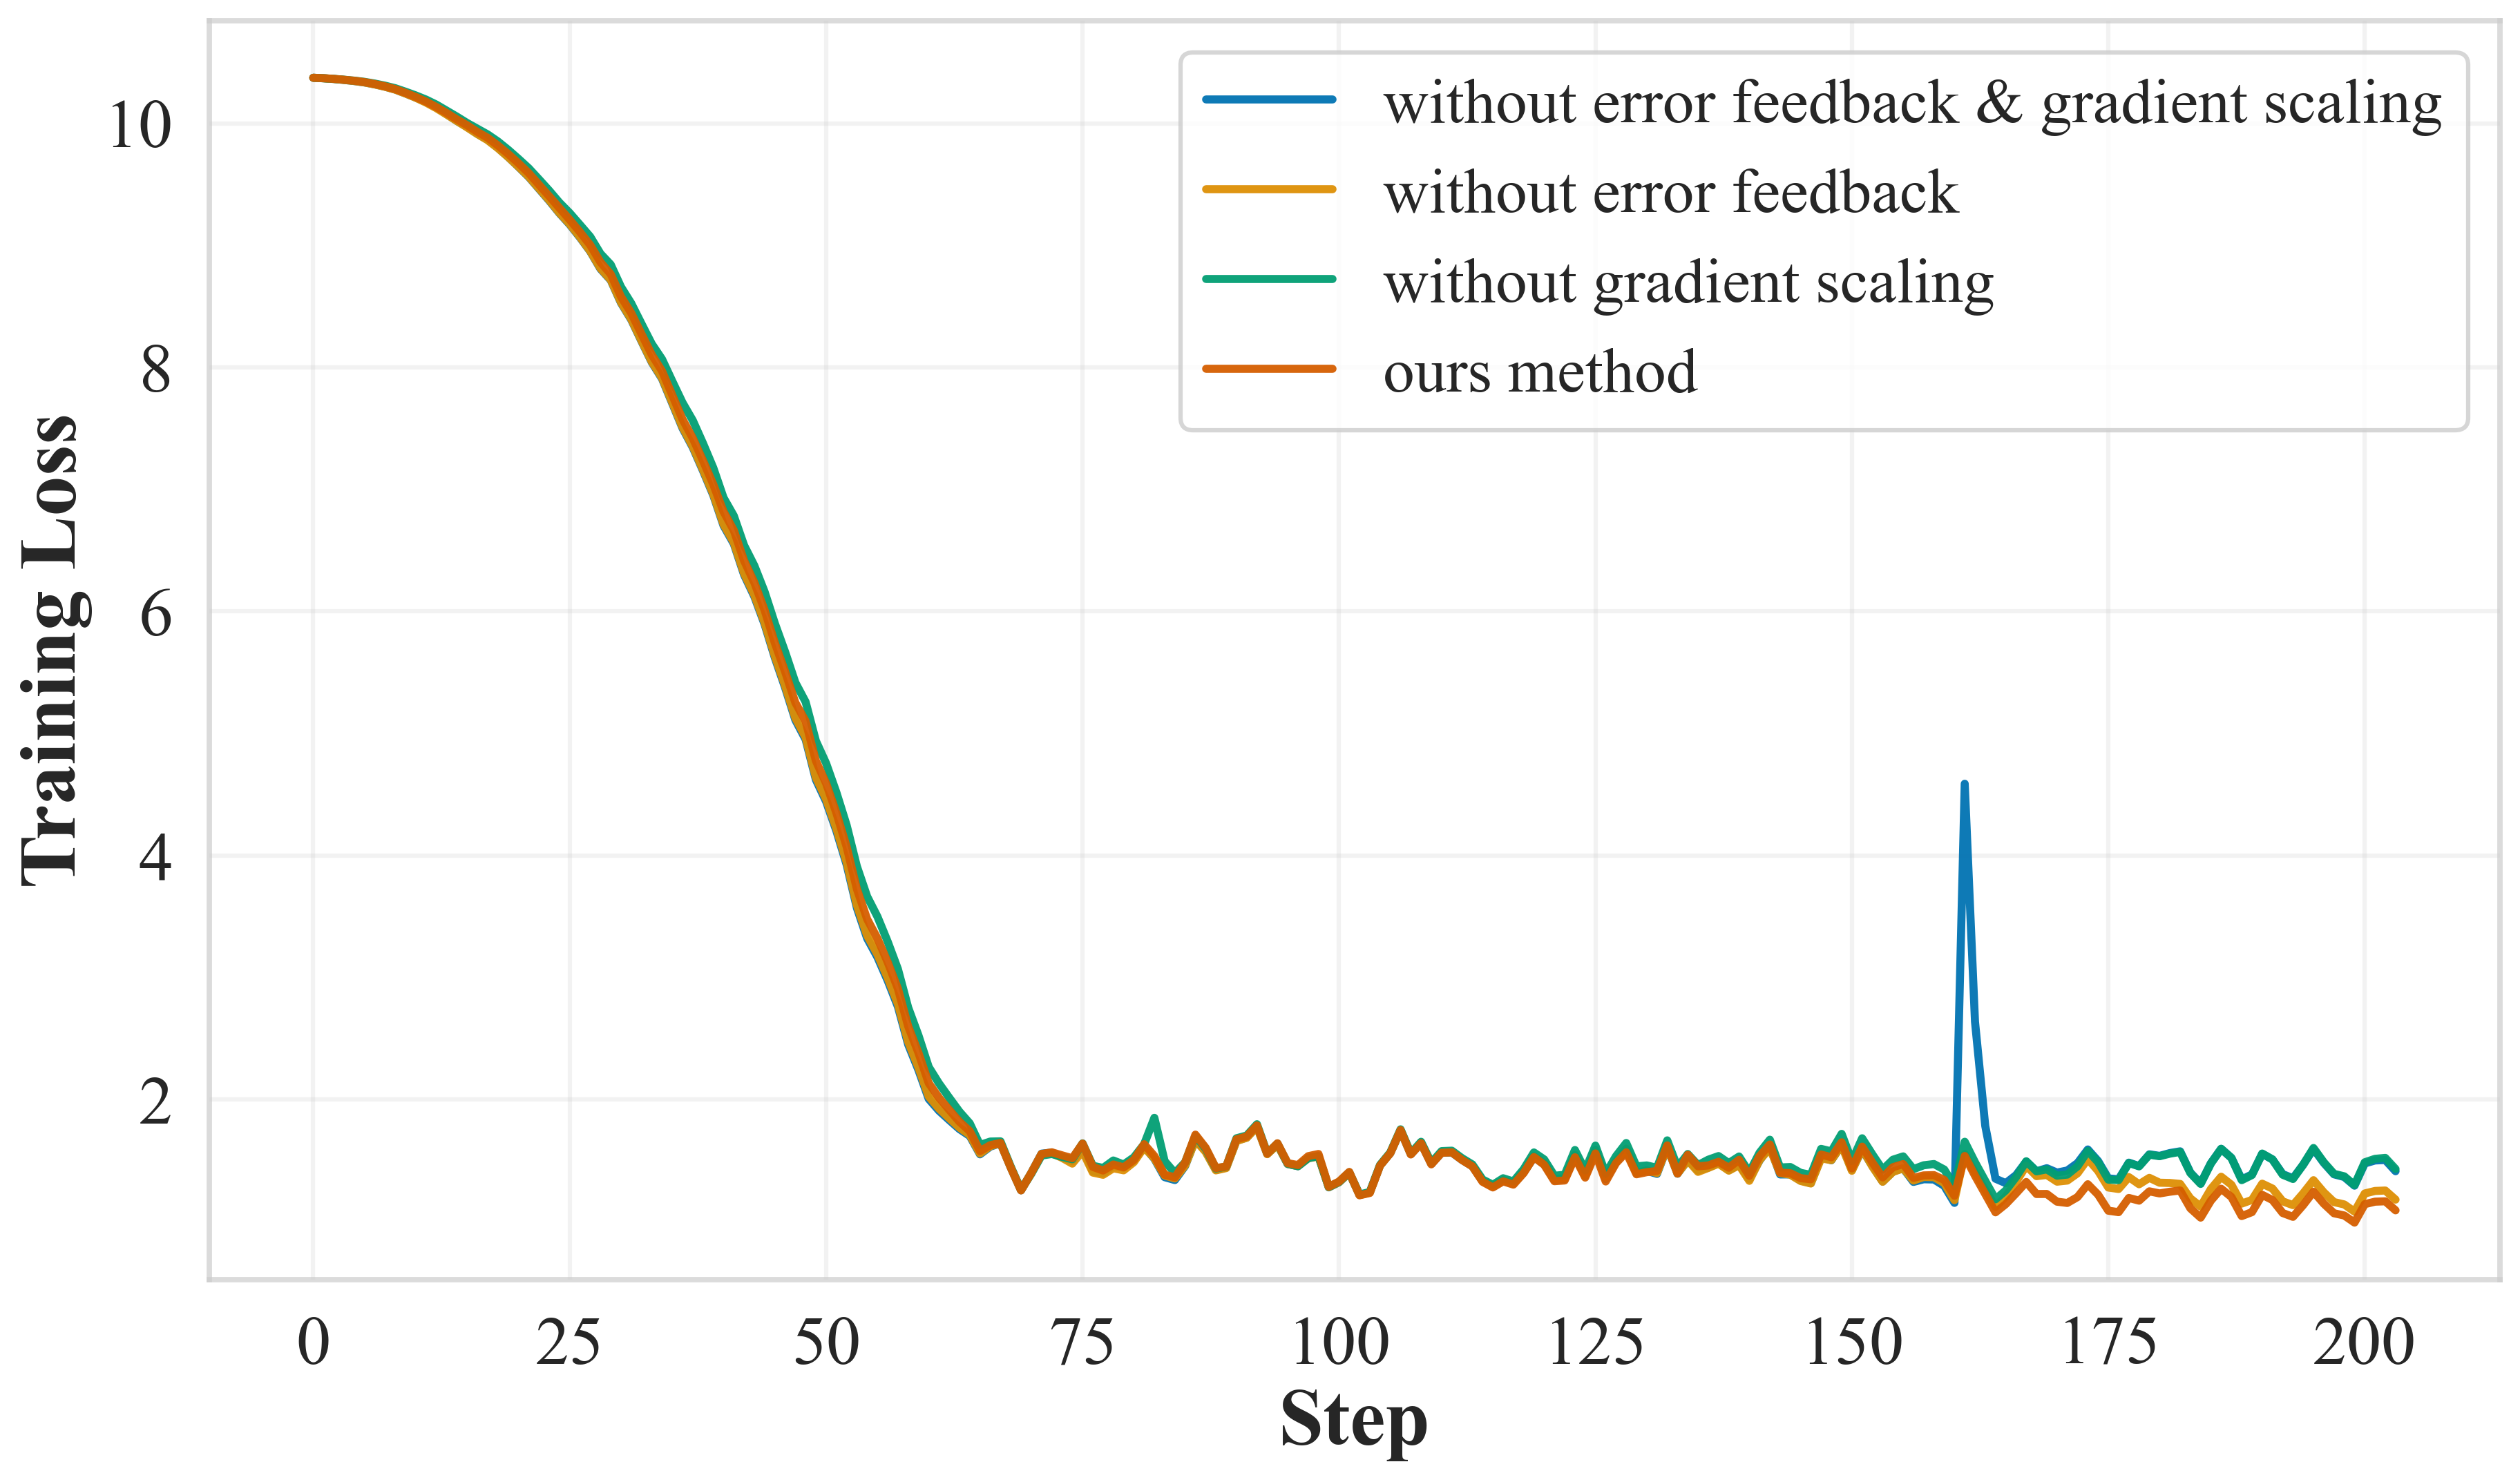
\includegraphics[width=\columnwidth]{images/json_curves_by_steps_ablation.png}
    \caption{Training loss changes with step under different ablation settings.}
    \label{fig:loss_ablation}
\end{figure}

% 我们针对本文的两个核心机制进行了消融实验，如\ref{fig:loss_ablation}所示，对于设置完全一致的训练，不使用gradient scaling方法，不使用error feedback策略，对于error feedback策略和gradient scaling策略都不使用这三个方法而言，相对于我们的原始方法在收敛程度、收敛稳定性上存在轻微的损失。对于不使用gradient scaling和error feedback方法而言，最终loss的收敛程度有所退化；而二者均不使用的情况下，在训练已经收敛的时候出现了明显的spike，预示着训练稳定性遭到了一定程度的挑战。

We conduct ablation experiments on the two core mechanisms of this paper. As shown in \ref{fig:loss_ablation}, for training with identical configurations, the three variants: without gradient scaling, without the error feedback strategy, and without both gradient scaling and error feedback exhibit a slight degradation in terms of convergence degree and convergence stability compared to our original method. Specifically, the variant without gradient scaling and error feedback shows a degraded convergence in the final loss. For the variant without both mechanisms, obvious spikes appear after training has converged, indicating that the stability of the training is compromised to some extent.

% \subsection{Analysis and Discussion}

% Overall, the two figures jointly indicate that POLAR-SGD preserves step-wise convergence behavior while substantially improving wall-clock convergence. Compared with relaxed-synchronization baselines, POLAR-SGD exhibits a more stable training trajectory and reaches the low-loss regime faster in time, making it a practical and effective solution for large-scale training under realistic WAN-constrained Cross-DC settings.

% \subsection{Main Results}

% \paragraph{Throughput Improvement.}

% On the LLaMA-2 7B pre-training task, POLAR-SGD demonstrates a significant performance advantage. Our method achieves a \textbf{1.87$\times$ end-to-end throughput improvement} compared to the Standard DP+PP baseline. This result strongly validates the effectiveness of eliminating the pipeline stall by overlapping communication and computation.

% Nsight system profiling reveals that the baseline spends 34\% of each training step idle while waiting for All-Reduce communication. In contrast, POLAR-SGD reduces this communication overhead to just 7\%, which is primarily incurred during the pipeline ramp-up and ramp-down phases where overlap is not fully possible. This corresponds to a \textbf{4.8× reduction in communication-induced idle time}.

% \textbf{Model Convergence Quality.}

% Performance gains should not come at the expense of model quality. Figure~\ref{fig:loss_comparison} shows the training loss and validation perplexity curves for POLAR-SGD and the baseline method. We observe that POLAR-SGD exhibits a slightly slower convergence in the initial training phase (first 400 steps), which is attributable to the gradient asynchrony introduced by pipelined communication. However, this difference is transient—after 400 steps, POLAR-SGD's convergence curve aligns perfectly with the Standard DP+PP baseline, ultimately achieving identical model quality.

% This result is significant: despite the slight initial convergence fluctuation, our predictive error-correction mechanism successfully guides the model back to the optimal convergence path, ensuring that final performance is not compromised. More importantly, given that POLAR-SGD provides a 1.87× throughput improvement throughout training, even with the slight initial convergence difference, its end-to-end training efficiency (measured by wall-clock time to reach a target loss) still far exceeds the baseline. In other words, while POLAR-SGD may require slightly more steps to reach a given loss value, the substantially reduced per-step time results in significantly lower total training time.

% \subsection{Convergence and Model Quality}

% \subsection{Ablation Study}

% To isolate and verify the necessity of the predictive error-correction (EC) mechanism, we conducted an ablation study. We compare the full POLAR-SGD method against the "Pipelined (w/o EC)" variant, which disables the correction mechanism.

% The results show that while the "Pipelined (w/o EC)" variant still achieves a performance benefit from pipelining, its model convergence is significantly impaired. On the WikiText-103 task, its final validation perplexity degraded from \textbf{10.38 (with POLAR-SGD) to 10.71}, a 3.2\% regression. This clearly demonstrates that without compensating for the gradient divergence introduced by asynchrony, the model deviates from the optimal convergence path, leading to a drop in final performance.

% This ablation study provides strong evidence that the predictive error-correction mechanism is an indispensable component of POLAR-SGD. It is the key that enables our aggressive communication overlap strategy to be practical, ensuring that the significant gains in throughput do not sacrifice the final model quality.

    \section{Related Work}
    
    \label{related-work}

This section situates \sysname{} with respect to the most relevant algorithmic and system approaches for distributed training limited by the WAN, focusing on precise differences in the mechanism and objectives.

\subsection{Local Updates / Local‑SGD}
Local‑SGD reduces global communication by executing multiple local SGD steps between periodic aggregations, which lowers aggregate bandwidth but induces ``client drift''~\cite{stich2019local, stich2018sparsified, compensatefedavg}. The sysname{} function does not primarily sparsify synchronization points; rather, it uses micro-batch granular continuous gradient transmission to avoid model drift.

\subsection{Gradient Compression and Error‑Feedback}
Quantization and sparsification combined with error feedback reduce transmitted bytes while recovering convergence guarantees under certain assumptions~\cite{DBLP:conf/dac/WangWLK25, zhang2023errorfeedback, zhou2023integrating, DBLP:conf/icml/XuH22}. Those techniques principally address bias from lossy encoding; \sysname{} addresses a distinct class of temporal misalignment errors arising from early transmission of gradients and is compatible with compression + error‑feedback applied on its continuous gradient stream.

\subsection{Overlap and Pipelining}
Overlap techniques and model‑parallel pipelining hide communication by interleaving compute and communication or by partitioning layers across devices~\cite{gpipe, pipedream, zerobubble}. While such methods can reduce on‑step communication tails, cross‑DC model pipelining typically requires activation transfers that are prohibitive in WAN environments; unlike opportunistic intra‑step overlap, \sysname{} proactively moves micro‑batch gradients out‑of‑band into a sustained background flow, avoiding cross‑DC activation transfer and converting bursty synchronization into steady, low‑jitter traffic.

\subsection{Summary and Positioning}
\sysname{} draws on three related lines of work: micro-batch/overlap techniques, asynchronous and delay-compensation methods, and error-feedback approaches. It departs from these prior lines in three principal ways: (i) it moves synchronization to micro-batch granularity; (ii) it employs predictive correction targeted at the temporal mismatch between previewed gradients and subsequent local updates. The empirical section evaluates \sysname{} against representative instances from these families in terms of throughput, convergence speed, and final accuracy under diverse WAN conditions and data heterogeneity.

% \textbf{Cross-datacenter / WAN training systems.}
% Training across geographically separated datacenters is fundamentally constrained by wide-area network (WAN) properties: lower bandwidth, higher latency, and higher variability than intra-datacenter fabrics. These characteristics make collective communication a first-order bottleneck, and can turn otherwise negligible synchronization into a dominant component of iteration time. As a result, Cross-DC training systems often adopt WAN-aware orchestration (e.g., topology-aware collectives and placement) and favor parallelism layouts that minimize cross-site traffic on the critical path. In particular, using data parallelism across sites avoids shipping activations across the WAN (as would happen if pipeline boundaries span datacenters), but it still requires frequent gradient aggregation across sites, leaving a recurring synchronization barrier to optimize.

% \textbf{Communication overlap, asynchronous optimization, and Local SGD.}
% A broad line of work improves throughput by overlapping gradient communication with backpropagation, for example by launching reductions for gradient buckets as soon as they are ready. While such overlap can hide a substantial portion of communication, the final ``tail'' of an iteration often remains on the critical path because some reductions must complete before the optimizer step. Relaxing synchronization further---via asynchronous or semi-asynchronous SGD---can remove global barriers but typically introduces stale gradients and may destabilize convergence. Local-update methods (often referred to as Local SGD / federated averaging) reduce synchronization frequency by performing multiple local steps between global aggregations; however, the remaining synchronization can still be expensive under WAN conditions, and increasing the local update window can lead to model drift and degraded quality. \sysname is complementary: rather than only reducing synchronization frequency, it restructures \emph{when} gradients are synchronized so that communication can proceed continuously in the background.

% \textbf{Error feedback, delayed-gradient correction, and pipelining.}
% There is extensive literature on mitigating optimization error introduced by delayed or approximate communication, including error-feedback mechanisms used with gradient compression, correction terms for delayed gradients. These methods share the principle of tracking the discrepancy between an ``ideal'' update and the update actually applied under system constraints, then feeding that discrepancy back into future updates. \sysname follows this lineage with a predictive error-correction mechanism tailored to micro-batch-level pipelining: gradients are communicated early to enable overlap, while a lightweight correction term compensates for the mismatch induced by applying updates out of phase with subsequent gradient computation. This positions \sysname as combining fine-grained pipelined synchronization with principled correction for WAN-constrained Cross-DC training.

    \section{Conclusion}
    
    \label{conclusion}

We presented POLAR-SGD, which pipelines gradient communication across micro-batches to overlap synchronization with computation, and stabilizes the resulting asynchrony via a lightweight predictive (error-feedback) correction mechanism.

In a realistic Cross-DC emulation (30~Gb/s bandwidth, 50~ms RTT) on LLaMA-2 7B with 32 A100 GPUs, POLAR-SGD improves training throughput by \textbf{1.87$\times$}, while model quality is successfully maintained comparable to the synchronous baseline.

% \paragraph{Limitations and future work.}
% Our experiments focus on a specific WAN regime and a DP-centric Cross-DC organization; extending POLAR-SGD to more heterogeneous multi-site deployments and to stronger network variability is an important next step.
% It is also promising to study how the approach interacts with other parallelism strategies and collectives (e.g., tensor/expert parallelism and their synchronization patterns), and to validate robustness at larger model and cluster scales.


\bibliography{bib}
\bibliographystyle{icml2026}

%%%%%%%%%%%%%%%%%%%%%%%%%%%%%%%%%%%%%%%%%%%%%%%%%%%%%%%%%%%%%%%%%%%%%%%%%%%%%%%
%%%%%%%%%%%%%%%%%%%%%%%%%%%%%%%%%%%%%%%%%%%%%%%%%%%%%%%%%%%%%%%%%%%%%%%%%%%%%%%
% APPENDIX
%%%%%%%%%%%%%%%%%%%%%%%%%%%%%%%%%%%%%%%%%%%%%%%%%%%%%%%%%%%%%%%%%%%%%%%%%%%%%%%
%%%%%%%%%%%%%%%%%%%%%%%%%%%%%%%%%%%%%%%%%%%%%%%%%%%%%%%%%%%%%%%%%%%%%%%%%%%%%%%
\newpage
\appendix
\onecolumn

\section{Additional Details}
\label{sec:appendix}

\subsection{Code base}
\label{app:code_base}
Our code is published at: \hyperlink{}{https://anonymous.4open.science/r/polar-sgd-7583}. 

\subsection{Rethinking Parallelism Choices in Cross-DC Training}
\label{app:rethink_parallelism}
We can make the above distinction precise by comparing how cross-datacenter communication scales with the global batch size $B$.

Consider $D$ datacenters, each processing local minibatch $b$ such that $B = D \cdot b$, and let $\alpha$ be bytes per parameter communicated. Let $A$ denote the bytes of activation tensors that must cross a pipeline boundary \emph{per sample} when a pipeline cut spans datacenters (this includes the forward activations and, correspondingly, backward activation gradients on the return path).

\textbf{Cross-DC DP (gradient synchronization).}
In data parallel training, each datacenter performs forward/backward locally and participates in a global gradient aggregation once per iteration. The amount of data communicated across datacenters for the aggregation is proportional to the model size, not the batch size:
\[
V_{\mathrm{DP}} \approx \alpha P
\]
Thus, with fixed model size, the WAN communication volume for DP is \emph{constant} as $B$ increases.

\textbf{Cross-DC PP (activation transfer).}
When pipeline stages are placed in different datacenters, each microbatch must transmit activations across the WAN at each cross-DC boundary. Aggregated over the iteration, the WAN traffic scales with the number of samples processed:
\[
V_{\mathrm{PP}} \approx \Theta(B \cdot A),
\]
meaning cross-DC PP incurs WAN communication that grows \emph{linearly} with the global batch size.

\textbf{Implication on iteration time and throughput.}
Let $\mathrm{BW}_{\mathrm{WAN}}$ be the effective WAN bandwidth and $\mathrm{Lat}_{\mathrm{WAN}}$ the WAN latency. A coarse lower bound on communication time is:
\[
T_{\mathrm{comm}} \approx \mathrm{Lat}_{\mathrm{WAN}} + \frac{V}{\mathrm{BW}_{\mathrm{WAN}}}.
\]
Therefore,
\begin{align*}
    T_{\mathrm{comm}}^{\mathrm{DP}} \approx \mathrm{Lat}_{\mathrm{WAN}} + \frac{\alpha P}{\mathrm{BW}_{\mathrm{WAN}}},\\
    T_{\mathrm{comm}}^{\mathrm{PP}} \approx \mathrm{Lat}_{\mathrm{WAN}} + \frac{c \, B A}{\mathrm{BW}_{\mathrm{WAN}}},
\end{align*}
where $c$ captures constants such as the number of cross-DC cuts and forward/backward directions.

As $B$ increases, $T_{\mathrm{comm}}^{\mathrm{PP}}$ increases proportionally, and more importantly, PP communication lies on the critical path due to stage ordering constraints, so WAN variability directly stalls compute. In contrast, $T_{\mathrm{comm}}^{\mathrm{DP}}$ does not grow with $B$; the compute per iteration typically increases with $B$, so the fixed WAN synchronization cost is amortized over more computation and samples. Consequently, end-to-end throughput of DP-centric Cross-DC training becomes increasingly favorable at large batch sizes, while PP-centric Cross-DC training suffers growing WAN overhead and sensitivity to network dynamics.

\subsection{Proofs}

We provide a convergence analysis showing that POLAR-SGD retains the same \emph{asymptotic} convergence behavior as synchronous SGD, up to an additional term controlled by the error-feedback residual.

\subsubsection{Assumptions}

We make the following standard assumptions in stochastic optimization:

\begin{assumption}[L-Smoothness]
\label{assump:smooth}
The loss function $f(w)$ is $L$-smooth, i.e., for all $w, w'$:
\begin{equation}
    \|\nabla f(w) - \nabla f(w')\| \leq L \|w - w'\|.
\end{equation}
\end{assumption}

\begin{assumption}[Unbiased Gradient]
\label{assump:unbiased}
For each worker $r$ and micro-batch $m$, the stochastic gradient is unbiased:
\begin{equation}
\mathbb{E}\left[g_{r,t,m}\mid w_t\right] = \nabla f(w_t).
\end{equation}
\end{assumption}

\begin{assumption}[Bounded Variance]
\label{assump:variance}
The variance of stochastic gradients is bounded:
\begin{equation}
\mathbb{E}\left[\|g_{r,t,m} - \nabla f(w_t)\|^2 \mid w_t\right] \le \sigma^2.
\end{equation}
\end{assumption}

\noindent
% \textbf{Remark.} Our analysis focuses on the DP synchronization effect introduced by prefix-based communication. The pipeline execution order does not change the definition of per-micro-batch stochastic gradients; gradients are accumulated normally over $M$ micro-batches within each iteration.

\subsubsection{Main Convergence Theorem}

\begin{theorem}[Convergence of POLAR-SGD (mean All-Reduce with error feedback)]
\label{thm:convergence}
Under Assumptions~\ref{assump:smooth}--\ref{assump:variance}, with learning rate $\eta \leq \frac{1}{2L}$, after $T$ global iterations, POLAR-SGD satisfies
\begin{equation}
\begin{aligned}
\frac{1}{T}\sum_{t=0}^{T-1}\mathbb{E}\left[\|\nabla f(w_t)\|^2\right]
\le\;&
\frac{2\big(f(w_0)-f^*\big)}{\eta T}
+ \frac{L\eta\sigma^2}{N}
\\
&+ \frac{L\eta}{T}\sum_{t=0}^{T-1}\mathbb{E}\left[\|\bar e_t\|^2\right],
\end{aligned}
\label{eq:main_bound}
\end{equation}
where $f^*=\inf_w f(w)$ and $\bar e_t=\frac{1}{N}\sum_{r=1}^N e_{r,t}$ is the averaged error buffer.
\end{theorem}

\subsection{Detailed Proof}
\label{app:proof}

\subsubsection{Key Definitions (Aligned with Algorithm 2)}
For a global iteration with $M$ micro-batches, we define:
\begin{itemize}
  \item $i$: Index of the micro-batch where communication is triggered ($1 \leq i \leq M$)
  \item $g_a^{(i)} = \sum_{k=1}^i g_{k}$: Local accumulated gradient from micro-batch 1 to $i$
  \item $g_{\text{pred}}^{(i)} = \frac{M}{i} \cdot g_a^{(i)}$: Predicted full-batch gradient (scaled by $\frac{M}{i}$ to match the norm of the full $M$ micro-batches)
  \item $e^{(i)} = g_a^{(M)} - g_{\text{pred}}^{(i)}$: Error buffer (compensation term for the unsynchronized micro-batches $i+1$ to $M$)
  \item $g_{\text{sync}}^{(i)} = \frac{1}{N}\sum_{j=1}^N \left(g_{\text{pred},j}^{(i)} + e_j^{(i-1)}\right)$: Global synchronized gradient (incorporating error feedback from the previous step)
\end{itemize}

\subsubsection{Assumptions (Revised for Asynchronous Scenarios)}
We retain the three standard assumptions and add one asynchronous bias constraint to match POLAR-SGD's pipeline communication:
\begin{enumerate}
  \item \textbf{$L$-Smoothness}: $\|\nabla f(w_1) - \nabla f(w_2)\| \leq L\|w_1 - w_2\|$ for all $w_1,w_2$
  \item \textbf{Unbiased Gradient}: $\mathbb{E}[g_{k} \mid w_k] = \nabla f(w_k)$, where $w_k$ is the parameter used for micro-batch $k$
  \item \textbf{Bounded Variance}: $\mathbb{E}\left[\|g_{k} - \nabla f(w_k)\|^2 \mid w_k\right] \leq \sigma^2$
  \item \textbf{Bounded Asynchronous Bias}: Due to pipeline communication, $w_k$ may differ from the globally synchronized parameter $w_{\text{sync}}$. We assume $\|w_k - w_{\text{sync}}\| \leq \Delta$, where $\Delta$ is a constant determined by communication-computation overlap ratio.
\end{enumerate}

\subsubsection{Proof Steps}
\textbf{Step 1: Error Buffer Dynamics and Boundedness}
The error buffer $e^{(i)}$ is defined as the deviation between the full local accumulated gradient $g_a^{(M)}$ and the predicted gradient $g_{\text{pred}}^{(i)}$ sent for synchronization:
\begin{equation}
e^{(i)} = \sum_{k=1}^M g_k - \frac{M}{i}\sum_{k=1}^i g_k = \sum_{k=i+1}^M g_k - \frac{M-i}{i}\sum_{k=1}^i g_k
\end{equation}

From the bounded variance assumption, each $g_k$ satisfies $\|g_k\| \leq G$ (a constant gradient norm bound for LLMs). Thus:
\begin{equation}
\|e^{(i)}\| \leq \sum_{k=i+1}^M \|g_k\| + \frac{M-i}{i}\sum_{k=1}^i \|g_k\| \leq M \cdot G
\end{equation}

This proves the boundedness of $e^{(i)}$: the error buffer has an upper bound $M \cdot G$ and lower bound $-M \cdot G$, which is independent of the number of global steps—it only depends on the number of micro-batches $M$ and the single micro-batch gradient norm $G$.

For multiple workers, the sum of errors across workers $\sum_{j=1}^N e_j^{(i)}$ is not necessarily zero—it depends on the randomness of local gradients across workers. However, due to the unbiasedness of local gradients, we can derive the expectation bound of the sum:
\begin{equation}
\mathbb{E}\left[\left\|\sum_{j=1}^N e_j^{(i)}\right\|^2\right] \leq N \cdot M^2 \cdot G^2
\end{equation}

\textbf{Step 2: Effective Gradient and Asynchronous Bias Compensation}
The global synchronized gradient incorporating error feedback is:
\begin{equation}
g_{\text{sync}}^{(i)} = \frac{1}{N}\sum_{j=1}^N \left(\frac{M}{i}g_{a,j}^{(i)} + e_j^{(i-1)}\right)
\end{equation}

Substitute $e_j^{(i-1)} = g_{a,j}^{(M)} - \frac{M}{i-1}g_{a,j}^{(i-1)}$ (from the previous step's error definition):
\begin{equation}
g_{\text{sync}}^{(i)} = \frac{1}{N}\sum_{j=1}^N \Bigg(\frac{M}{i}g_{a,j}^{(i)} + g_{a,j}^{(M)} - \frac{M}{i-1}g_{a,j}^{(i-1)}\Bigg)
\end{equation}

When $i = M$ (synchronization after all micro-batches), the predicted gradient equals the full local gradient, so $e_j^{(M)} = 0$. For general $i$, the effective gradient $g_{\text{sync}}^{(i)}$ can be rewritten as:
\begin{equation}
g_{\text{sync}}^{(i)} = \frac{1}{N}\sum_{j=1}^N g_{a,j}^{(M)} + \delta^{(i)}
\end{equation}
where $\delta^{(i)}$ is the asynchronous bias term caused by early synchronization. From the boundedness of $e^{(i)}$, we have $\|\delta^{(i)}\| \leq C \cdot \Delta$ (a constant $C$ related to $M$).

\textbf{Step 3: Iteration Inequality Under Smoothness}
The parameter update rule for POLAR-SGD is:
\begin{equation}
w^{(m+1)} = w^{(m)} - \eta \cdot g_{\text{sync}}^{(i,m)}
\end{equation}
where $g_{\text{sync}}^{(i,m)}$ is the synchronized gradient for micro-batch $m$ in the global iteration.

By $L$-smoothness:
\begin{equation}
f(w^{(m+1)}) \leq f(w^{(m)}) + \langle \nabla f(w^{(m)}), w^{(m+1)} - w^{(m)} \rangle + \frac{L}{2}\|w^{(m+1)} - w^{(m)}\|^2
\end{equation}

Substitute the update rule and expand:
\begin{equation}
f(w^{(m+1)}) \leq f(w^{(m)}) - \eta \langle \nabla f(w^{(m)}), g_{\text{sync}}^{(i,m)} \rangle + \frac{L\eta^2}{2}\|g_{\text{sync}}^{(i,m)}\|^2
\end{equation}

\textbf{Step 4: Expectation and Convergence Bound}
Take expectation over gradient randomness and asynchronous bias:
\begin{equation}
\mathbb{E}[f(w^{(m+1)})] \leq \mathbb{E}[f(w^{(m)})] - \eta \mathbb{E}\left[\langle \nabla f(w^{(m)}), g_{\text{sync}}^{(i,m)} \rangle\right] + \frac{L\eta^2}{2}\mathbb{E}\left[\|g_{\text{sync}}^{(i,m)}\|^2\right]
\end{equation}

From the unbiased gradient assumption and bounded asynchronous bias:
\begin{equation}
\mathbb{E}\left[\langle \nabla f(w^{(m)}), g_{\text{sync}}^{(i,m)} \rangle\right] = \|\nabla f(w^{(m)})\|^2 + \mathbb{E}\left[\langle \nabla f(w^{(m)}), \delta^{(i,m)} \rangle\right] \geq \|\nabla f(w^{(m)})\|^2 - D \cdot \Delta
\end{equation}
where $D$ is the Lipschitz constant of $\nabla f$.

For the second moment term, using bounded variance and error boundedness:
\begin{equation}
\mathbb{E}\left[\|g_{\text{sync}}^{(i,m)}\|^2\right] \leq \|\nabla f(w^{(m)})\|^2 + \frac{\sigma^2}{N} + C^2 \cdot \Delta^2
\end{equation}

Substitute back into the iteration inequality and rearrange:
\begin{equation}
\mathbb{E}[f(w^{(m+1)})] \leq \mathbb{E}[f(w^{(m)})] - \eta\left(1 - \frac{L\eta}{2}\right)\|\nabla f(w^{(m)})\|^2 + \eta D \Delta + \frac{L\eta^2}{2}\left(\frac{\sigma^2}{N} + C^2 \Delta^2\right)
\end{equation}

Set the learning rate condition $\eta \leq \frac{1}{2L}$ to ensure the coefficient of $\|\nabla f(w^{(m)})\|^2$ is positive:
\begin{equation}
1 - \frac{L\eta}{2} \geq \frac{3}{4}
\end{equation}

\textbf{Step 5: Summing Over Steps and Final Convergence Bound}
Sum over $M$ micro-batches per global iteration and $T$ global iterations:
\begin{equation}
\sum_{t=0}^{T-1}\sum_{m=0}^{M-1} \mathbb{E}\left[\|\nabla f(w_t^{(m)})\|^2\right] \leq \frac{4}{\eta}\Bigg(f(w_0) - f^* + T M \left(\eta D \Delta + \frac{L\eta^2}{2}\left(\frac{\sigma^2}{N} + C^2 \Delta^2\right)\right)\Bigg)
\end{equation}

Divide both sides by $TM$ to get the average gradient norm bound:
\begin{equation}
\frac{1}{TM}\sum_{t=0}^{T-1}\sum_{m=0}^{M-1} \mathbb{E}\left[\|\nabla f(w_t^{(m)})\|^2\right] \leq \frac{4(f(w_0) - f^*)}{\eta TM} + 4 D \Delta + \frac{2 L \eta}{N}\sigma^2 + 2 L \eta C^2 \Delta^2
\end{equation}

Set the learning rate $\eta = \frac{K}{\sqrt{TM}}$ (to balance convergence rate and bias) where $K \leq \frac{\sqrt{TM}}{2L}$. The convergence rate is $O(1/\sqrt{TM})$, which matches standard synchronous SGD. The additional terms ($4D\Delta$, $2L\eta C^2\Delta^2$) are constants determined by asynchronous bias, which vanish as $\Delta \to 0$ (full communication-computation overlap).

This completes the proof.
\label{app:exp_details}

%%%%%%%%%%%%%%%%%%%%%%%%%%%%%%%%%%%%%%%%%%%%%%%%%%%%%%%%%%%%%%%%%%%%%%%%%%%%%%%
%%%%%%%%%%%%%%%%%%%%%%%%%%%%%%%%%%%%%%%%%%%%%%%%%%%%%%%%%%%%%%%%%%%%%%%%%%%%%%%

\end{document}

% This document was modified from the file originally made available by
% Pat Langley and Andrea Danyluk for ICML-2K. This version was created
% by Iain Murray in 2018, and modified by Alexandre Bouchard in
% 2019 and 2021 and by Csaba Szepesvari, Gang Niu and Sivan Sabato in 2022.
% Modified again in 2023 and 2024 by Sivan Sabato and Jonathan Scarlett.
% Previous contributors include Dan Roy, Lise Getoor and Tobias
% Scheffer, which was slightly modified from the 2010 version by
% Thorsten Joachims & Johannes Fuernkranz, slightly modified from the
% 2009 version by Kiri Wagstaff and Sam Roweis's 2008 version, which is
% slightly modified from Prasad Tadepalli's 2007 version which is a
% lightly changed version of the previous year's version by Andrew
% Moore, which was in turn edited from those of Kristian Kersting and
% Codrina Lauth. Alex Smola contributed to the algorithmic style files.
